\section{Experiments}\label{sec:experiment}
We experimentally evaluated the performance and quality of our methodology (heuristic algorithm in \cref{subsec:heuristics}), and compared it against the exhaustive approach in~\cref{sec:nphard}. In the following,
\cref{subsec:experiments_infrastructure} presents the simulator and experimental settings used in our experiments;
%, as well as the complete experimental settings;
\cref{subsec:experiments_performance} analyses the performance of our solution in terms of execution time; \cref{subsec:experiments_quality} discusses the quality of the best pipeline instance generated by our solution according to the metrics $M_J$ and $M_{JSD}$ in \cref{subsec:metrics}.

\subsection{Testing Infrastructure and Experimental Settings}\label{subsec:experiments_infrastructure}
Our testing infrastructure is a Swift-based simulator of a service-based ecosystem, including service execution, selection, and composition.
The simulator first defines the pipeline template as a sequence of vertices, with $l$ the length of the pipeline template, and defines the size \windowsize\ of the sliding window, such that \windowsize$\leq$$l$.
    We recall that alternative vertices are modeled in different pipeline templates, while parallel vertices are not considered in our experiments since they only add a fixed execution time that is negligible and do not affect the performance and quality of our solution.
    Each vertex is associated with a (set of) policy that applies a filtering transformation that remove a given percentage of data.

    The simulator then starts the instantiation process.
    At each step $i$, it selects the subset \{\vi{i},$\ldots$,$v_{\windowsize+i-1}$\} of vertices with their corresponding candidate services, and generates all possible service combinations.
    The simulator calculates quality $Q$ for all combinations and instantiates \vi{i} with service \sii{i} from the optimal combination with maximum $Q$.
    The window is shifted by 1 (i.e., $i$=$i$+1) and the instantiation process restarts.
    When the sliding window reaches the end of the pipeline template, that is, $v_{\windowsize+i-1}$$=$$\vi{l}$, the simulator computes the optimal service combination and instantiates the remaining vertices with the corresponding services.
    Figure~\ref{fig:execution_example} shows an example of a simulator execution with $i$$=$2 and \windowsize$=$3. Subset \{\vi{2},\vi{3},\vi{4}\} is selected, all combinations generated, and corresponding quality $Q$ calculated.
  Optimal service combination \{\sii{11},\sii{22},\sii{31}\} is retrieved and \vii{2} in the pipeline instance instantiated with \sii{11}.

  The simulator defines dependencies between filtering transformations made by candidate services at consecutive vertices of the pipeline template.
  To this aim, it assigns a dependency rate to each service \si{i} modeling the amount of the filtering transformation done at \si{i} that overlaps the one at \si{i-1}.
  For example, let us consider the pairs of services (\si{11},\si{21}) and (\si{11},\si{22}) with the following configurations: \emph{i)} service \si{11} introduces a filtering transformation that removes the 20\% of the dataset, \emph{ii)} service \si{21} introduces a filtering transformation that removes 10\% of the dataset and has dependency rate equal to 1, meaning that the filtering transformation made by \si{21} completely overlaps the one made by \si{11}, \emph{iii)} service \si{22} introduces a filtering transformation that removes 5\% of the dataset and has dependency rate equal to 0.5, meaning that the filtering transformation made by \si{22} overlaps half of the one made by \si{11}. Jaccard Metric $M_{J_{21}}$$=$0.8 at service \si{21}; $M_{J_{22}}$$=$0.75 at \si{22}, showing how dependencies can the pipeline quality and, in turn, the instantiation process.

  Our experiments have been run on a virtual machine equipped with a Intel(R) Xeon(R) CPU E5-2620 v4 @ 2.10GHz CPU and 32GB RAM.
  Each experiment was repeated 10 times and the results averaged to improve the reliability of findings.

  \begin{figure}[!t]
    \centering
    \resizebox{0.7\columnwidth}{!}{%
      \begin{tikzpicture}[framed]


        \node[draw, circle, fill=gray!20,minimum width=0.8cm] (v1) at (1,5.2) {$\vi{1}$};
        \node[draw, circle, fill=gray!20,minimum width=0.8cm] (v2) at (3,5.2) {$\vi{2}$};
        \node[draw, circle, fill=gray!20,minimum width=0.8cm] (v3) at (5,5.2) {$\vi{3}$};
        \node[draw, circle, fill=gray!20,minimum width=0.8cm] (v4) at (7,5.2) {$\vi{4}$};
        \node[draw, circle, fill=gray!20,minimum width=0.8cm] (v5) at (9,5.2) {$\vi{5}$};
        \node[above, shift=({0,0.5}),  ] at (v3.north)  {Sliding Window};

        \node[draw, rectangle,fill=red!20] (s1) at (1,3.4) {$\sii{1}$};
        \node[draw, rectangle, fill=green!20] (s2) at (1,1.7) {$\sii{2}$};
        \node[draw, rectangle, fill=red!20] (s3) at (1,0) {$\sii{3}$};

        \node[draw, rectangle,thick] (s11) at (3,3.4) {$\sii{11}$};
        \node[draw, rectangle,opacity=.6] (s12) at (3,1.7) {$\sii{12}$};
        \node[draw, rectangle,opacity=.6] (s13) at (3,0) {$\sii{13}$};

        \node[draw, rectangle,opacity=.6] (s21) at (5,3.4) {$\sii{21}$};
        \node[draw, rectangle,thick] (s22) at (5,1.7) {$\sii{22}$};
        \node[draw, rectangle,opacity=.6] (s23) at (5,0) {$\sii{23}$};

        \node[draw, rectangle, thick] (s31) at (7,3.4) {$\sii{31}$};
        \node[draw, rectangle,opacity=.6] (s32) at (7,1.7) {$\sii{32}$};
        \node[draw, rectangle,opacity=.6] (s33) at (7,0) {$\sii{33}$};

        \node[draw, rectangle] (s41) at (9,3.4) {$\sii{41}$};
        \node[draw, rectangle] (s42) at (9,1.7) {$\sii{42}$};
        \node[draw, rectangle] (s43) at (9,0) {$\sii{43}$};



        % \draw[->] (node2) -- (node3);
        % \draw[->] (s1) -- (s11);
        %\draw[->] (s2) -- (s12);
        % \draw[->] (s3) -- (s13);

        % \draw[->] (s1) -- (s11);
        % \draw[->] (s1) -- (s12);
        % \draw[->] (s1) -- (s13);

        \draw[->,line width= 0.7pt] (s2) -- (s11);
        \draw[->,dashdotted] (s2) -- (s12);
        \draw[->,dashdotted] (s2) -- (s13);

        \draw[->,line width= 0.7pt] (s11) -- (s22);
        % \draw[->,dashdotted] (s2) -- (s12);
        % \draw[->,dashdotted] (s2) -- (s13);

        \draw[->,dashdotted] (s11) -- (s21);
        \draw[->,dashdotted] (s11) -- (s23);

        \draw[->,dashdotted] (s12) -- (s21);
        \draw[->,dashdotted] (s12) -- (s22);
        \draw[->,dashdotted] (s12) -- (s23);

        \draw[->,dashdotted] (s13) -- (s21);
        \draw[->,dashdotted] (s13) -- (s22);
        \draw[->,dashdotted] (s13) -- (s23);


        \draw[->,dashdotted] (s21) -- (s31);
        \draw[->,dashdotted] (s21) -- (s32);
        \draw[->,dashdotted] (s21) -- (s33);

        \draw[->,line width=0.7pt] (s22) -- (s31);
        \draw[->,dashdotted] (s22) -- (s32);
        \draw[->,dashdotted] (s22) -- (s33);


        \draw[->,dashdotted] (s23) -- (s31);
        \draw[->,dashdotted] (s23) -- (s32);
        \draw[->,dashdotted] (s23) -- (s33);

        \draw[->] (v1) -- (v2);
        \draw[->] (v2) -- (v3);
        \draw[->] (v3) -- (v4);
        \draw[->] (v4) -- (v5);



        \begin{scope}[on background layer]
          \draw[thick, dashed, fill=red!10, opacity=0.5]
          ([shift={(-0.5,0.5)}]s11.north west) rectangle ([shift={(0.5,-0.5)}]s33.south east);



        \end{scope}
        \begin{scope}[on background layer]
          \draw[thick, dashed, fill=red!10, opacity=0.5]
          ([shift={(-0.5,0.5)}]v2.north west) rectangle ([shift={(0.5,-0.5)}]v4.south east);

        \end{scope}

        % \node[align = center, below,yshift=-20pt ] at (s23.south) {\ttfamily \scriptsize vertices=5  services=3  \windowsize=3  i=1};

      \end{tikzpicture}
    }
    \caption{Execution example of the sliding window heuristic using v=5, s=3, \windowsize=3 at i=1 step.}
    \label{fig:execution_example}
  \end{figure}

  \subsection{Perfomance}\label{subsec:experiments_performance}
  We first measured the performance (execution time) of our exhaustive and heuristic solutions by varying the number of vertices in the pipeline template from 2 to 7 and the number of services per vertex from 2 to 7. \cref{fig:time_window_perce_average} presents our results for both the exhaustive and heuristic solutions.
  The exhaustive approach is able to provide the optimal solution for all configurations, but its execution time grows exponentially with the number of vertices and services, making it impractical for large instances. For \windowsize from 1 to 3 (step 1), we observed a substantial reduction in execution time, with the heuristic always able to produce an instance in less than $\approx2.7\times10^5ms$ . The worst heuristic performance (7 vertices, 7 services, \windowsize=6) is $\approx3.8\times10^7ms$ is still one order of magnitude lower than the best exhaustive performance (7 vertices, 7 services, \windowsize=7) $\approx1.35\times10^8ms$.
  \begin{figure}[!htb]
    \centering
    \begin{subfigure}{0.45\textwidth}
      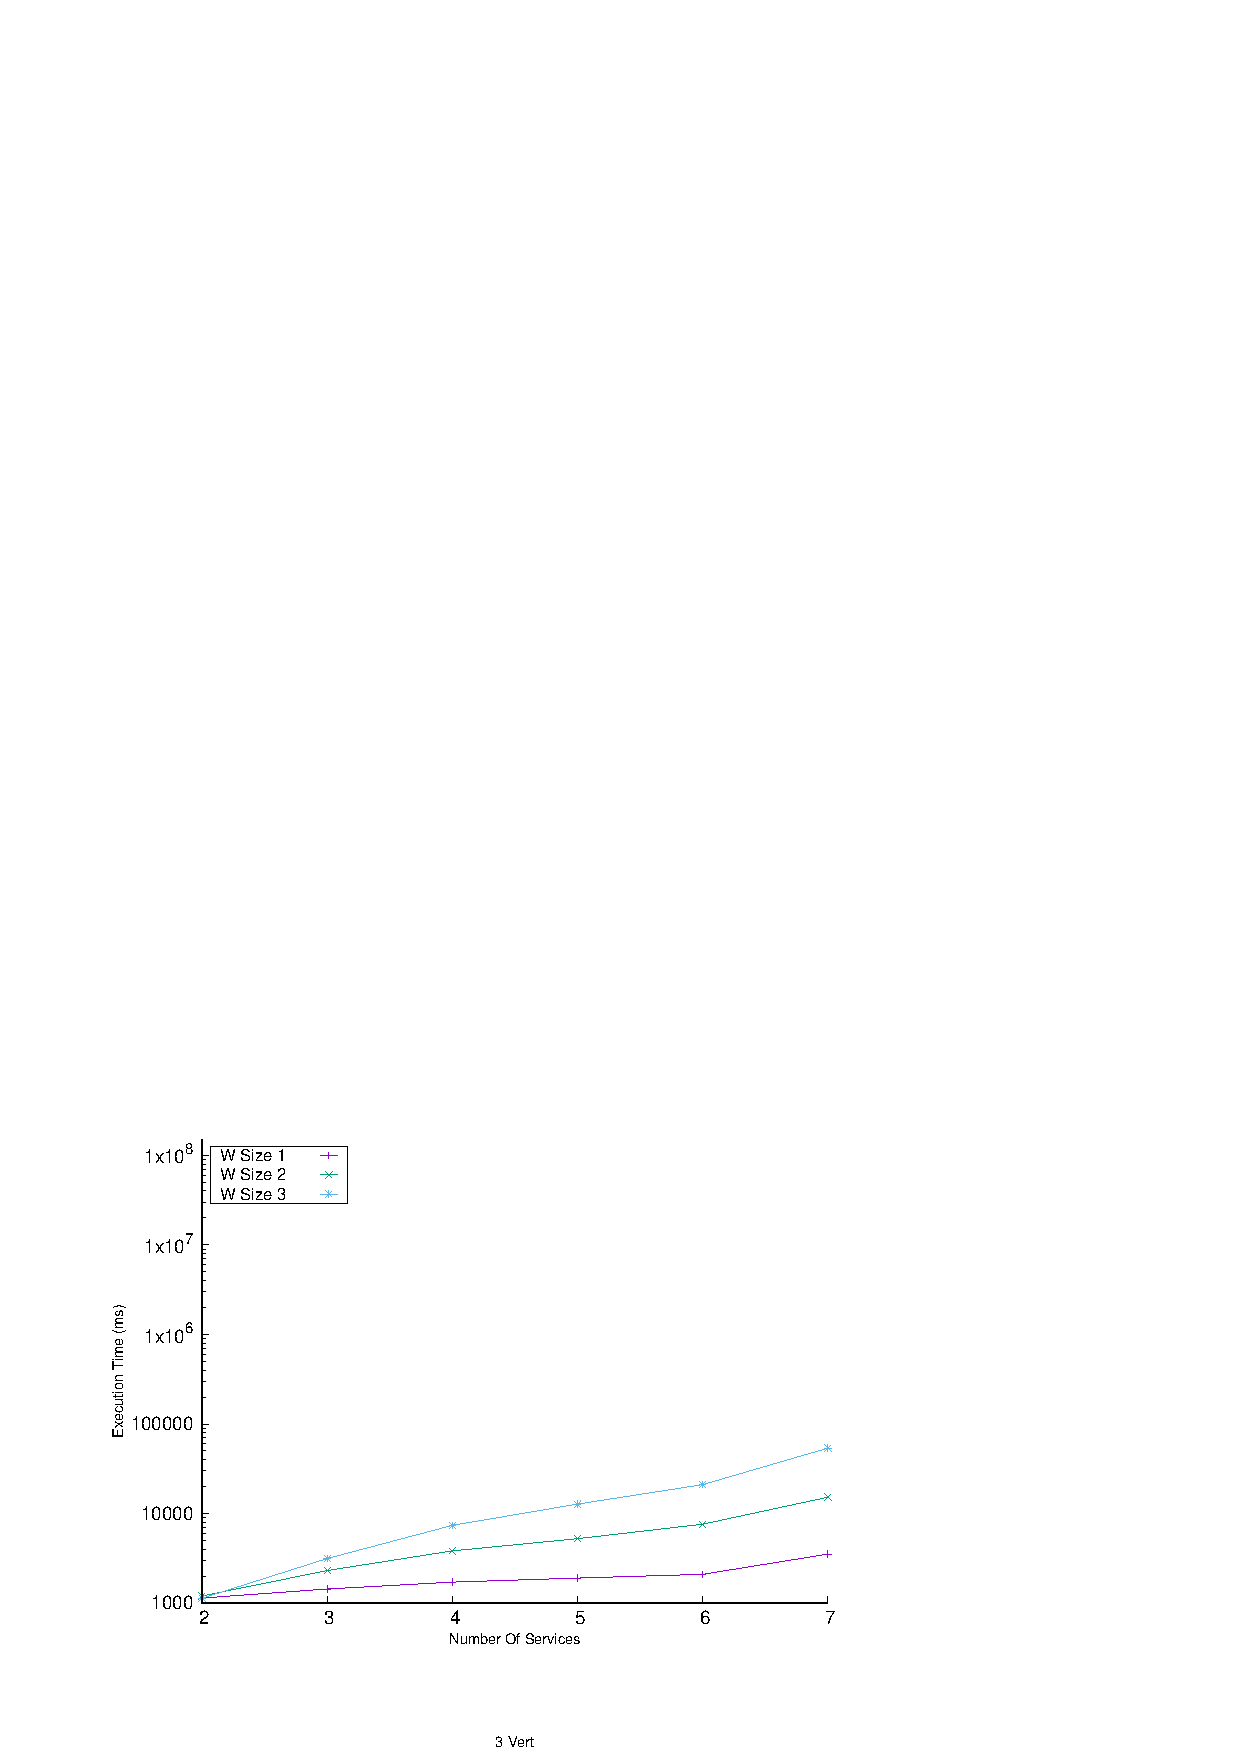
\includegraphics[width=\textwidth]{Images/graphs/window_time_performance_qualitative_n7_s7_50_80_n3}
      \caption{3 vertices}
      \label{fig:time_window_perce_wide_3n}
    \end{subfigure}
    \hfill
    \begin{subfigure}{0.45\textwidth}
      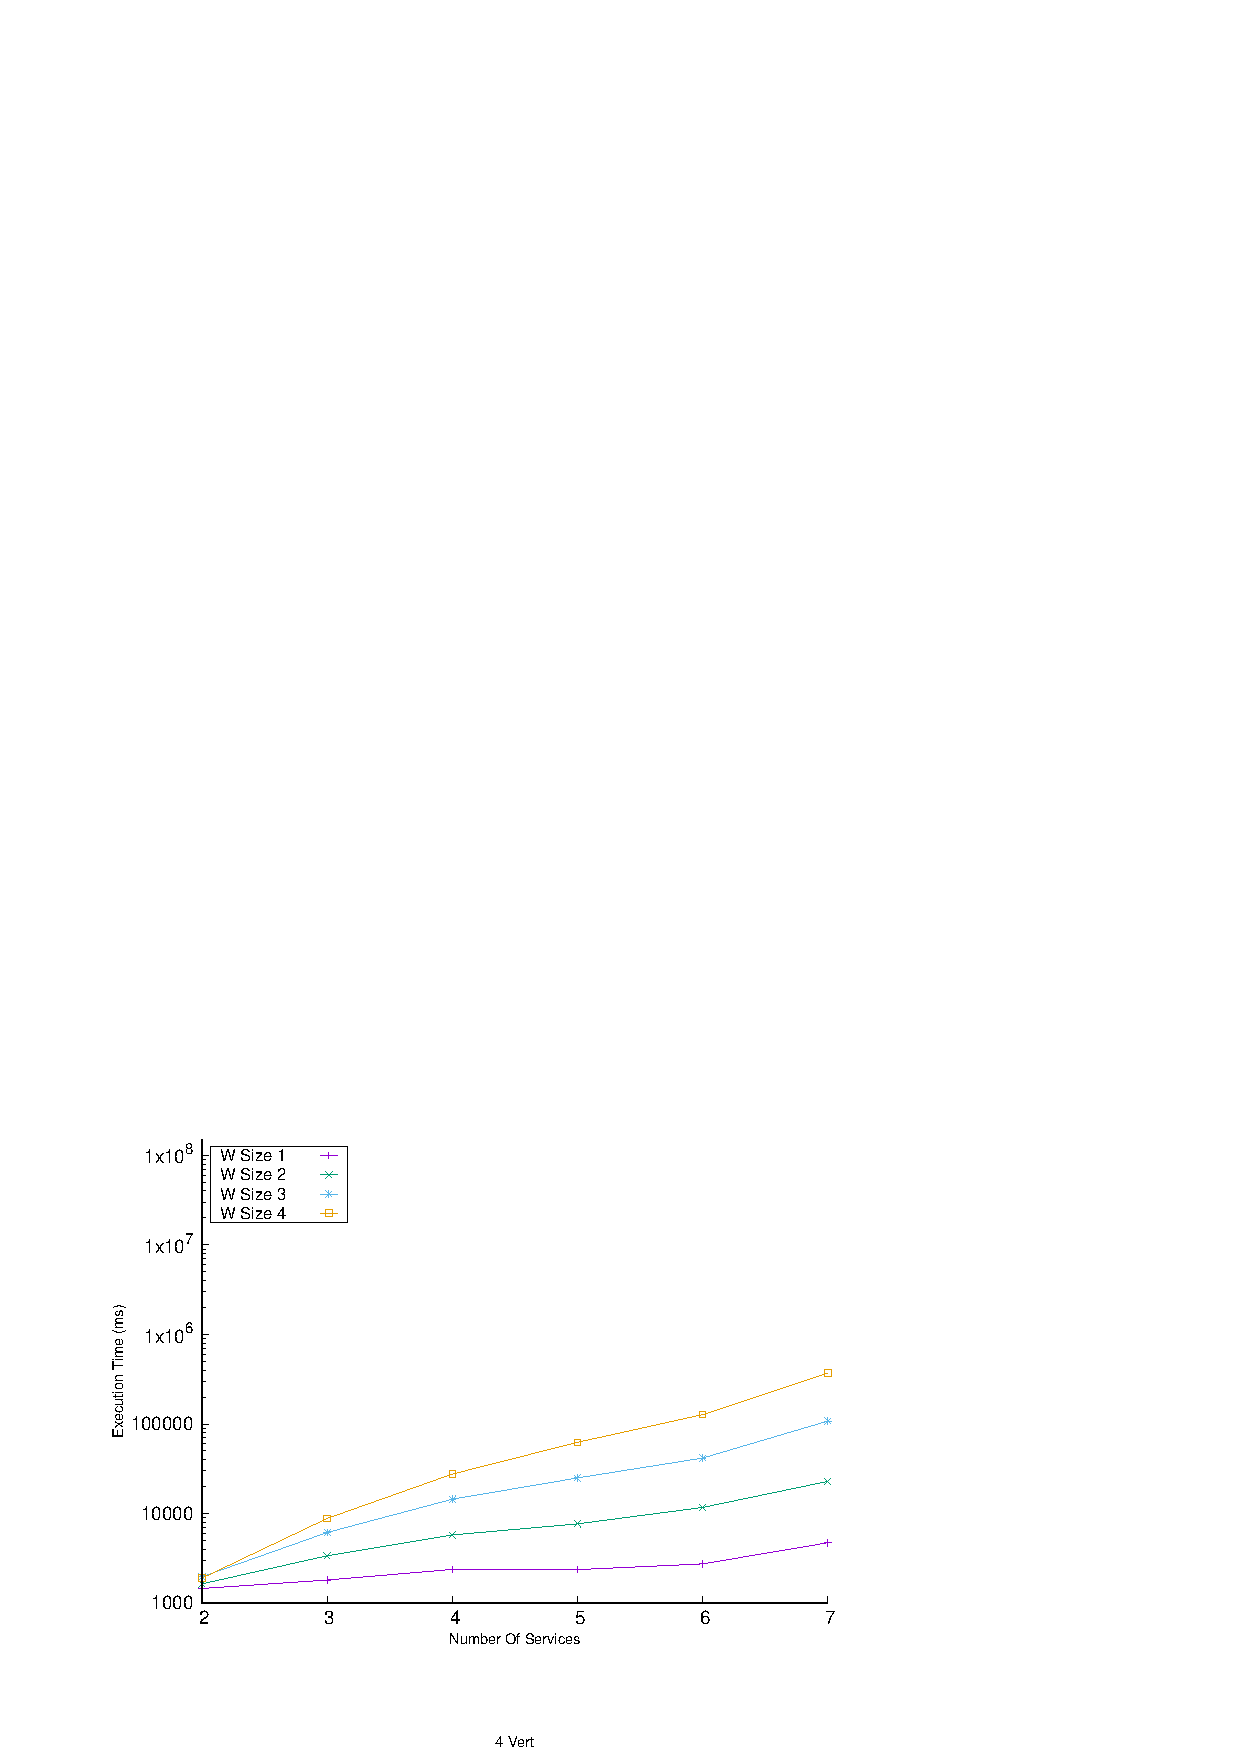
\includegraphics[width=\textwidth]{Images/graphs/window_time_performance_qualitative_n7_s7_50_80_n4}
      \caption{4 vertices}
      \label{fig:time_window_perce_wide_4n}
    \end{subfigure}
    \hfill
    \begin{subfigure}{0.45\textwidth}
      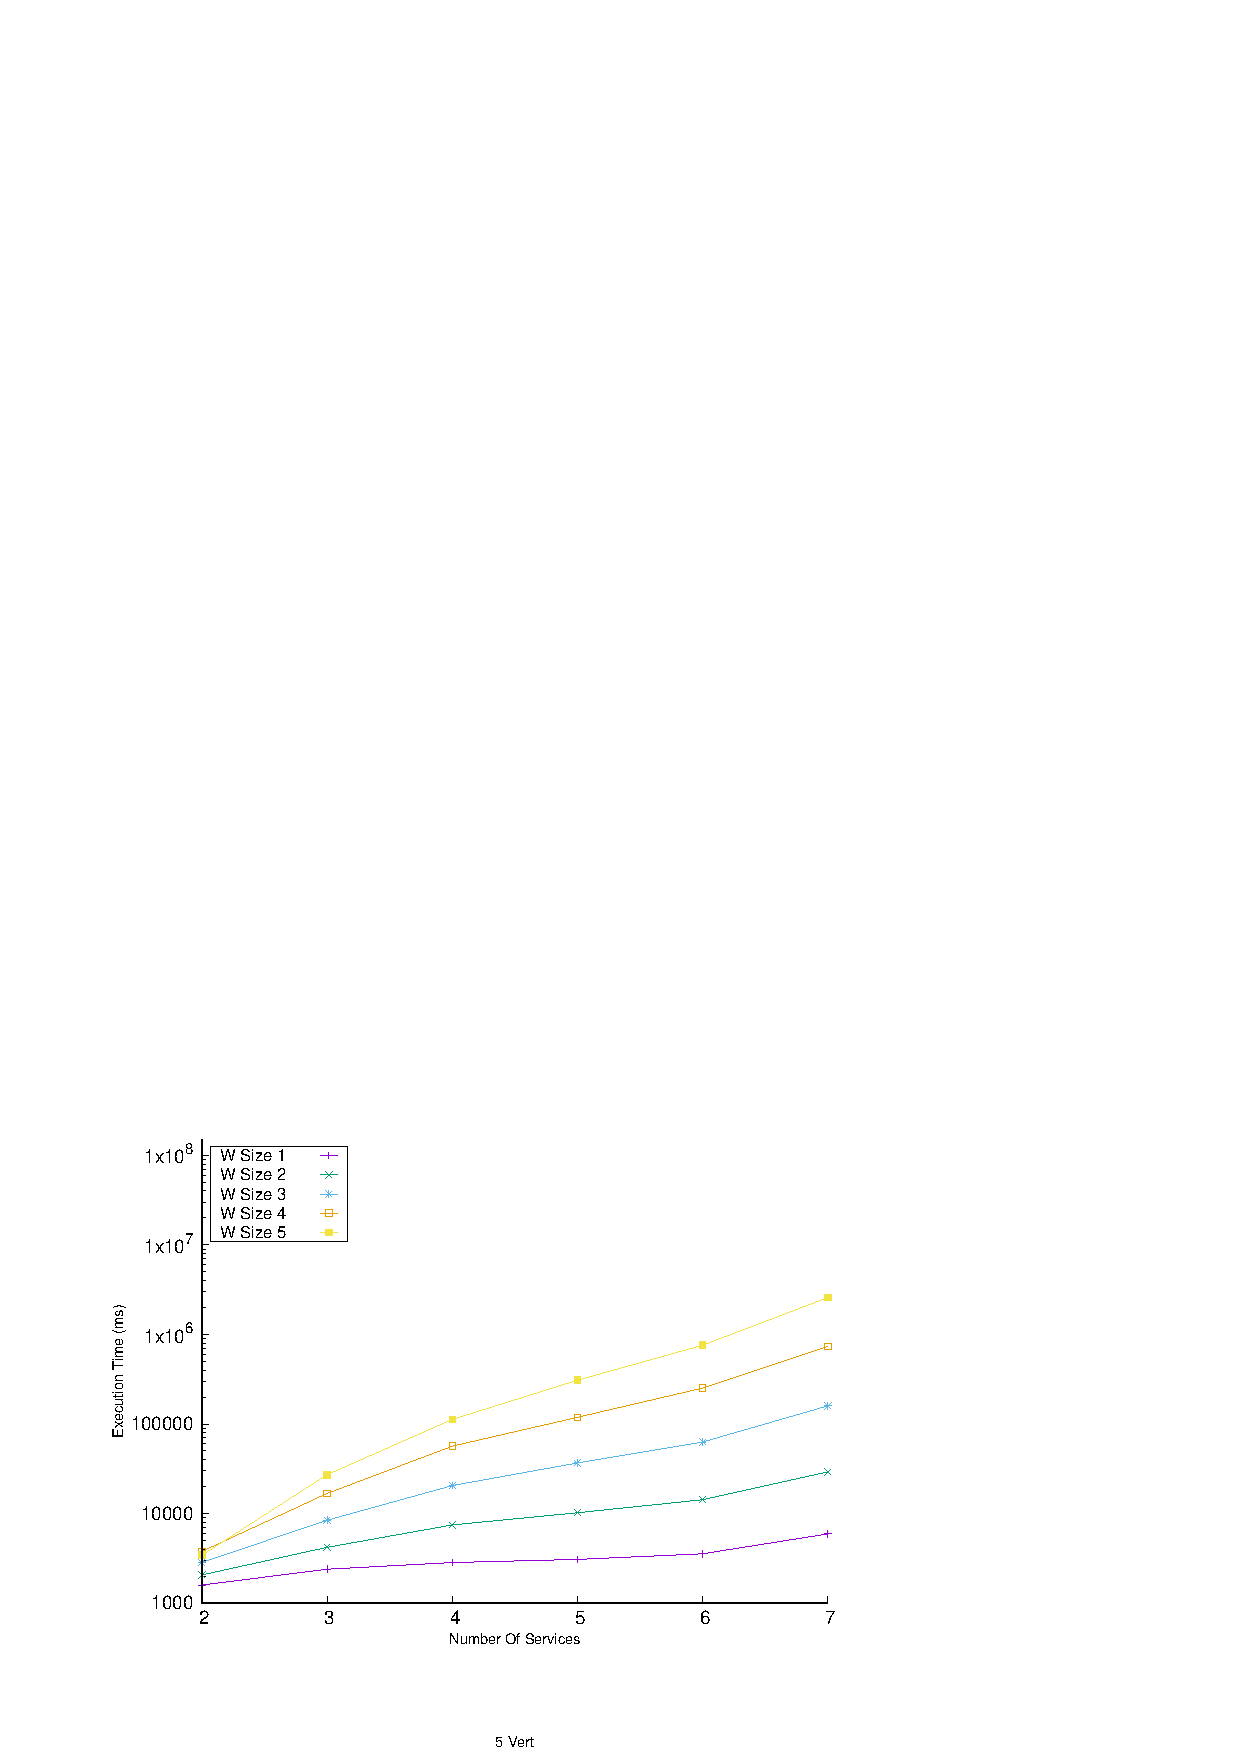
\includegraphics[width=\textwidth]{Images/graphs/window_time_performance_qualitative_n7_s7_50_80_n5}
      \caption{5 vertices}
      \label{fig:time_window_perce_wide_5n}
    \end{subfigure}
    \hfill
    \begin{subfigure}{0.45\textwidth}
      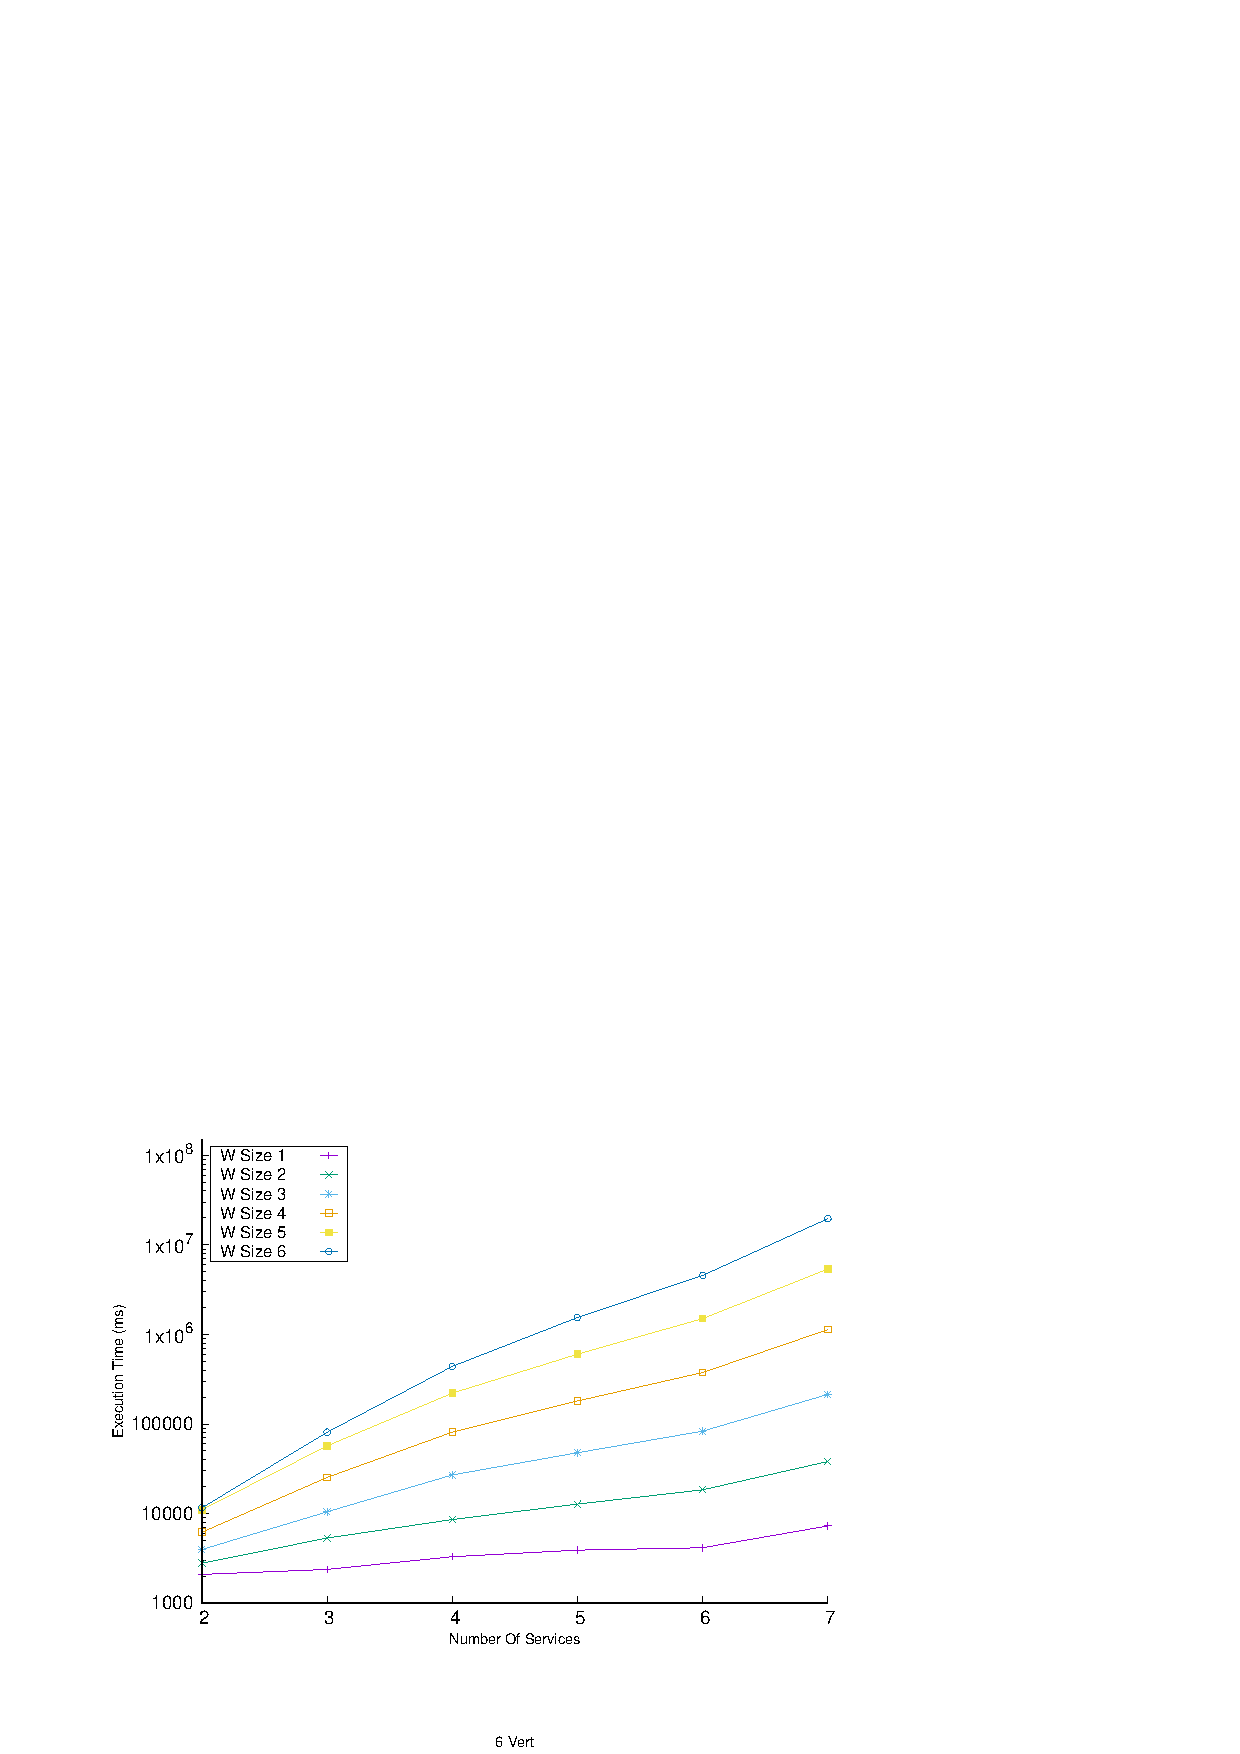
\includegraphics[width=\textwidth]{Images/graphs/window_time_performance_qualitative_n7_s7_50_80_n6}
      \caption{6 vertices}
      \label{fig:time_window_perce_wide_6n}
    \end{subfigure}
    \begin{subfigure}{0.45\textwidth}
      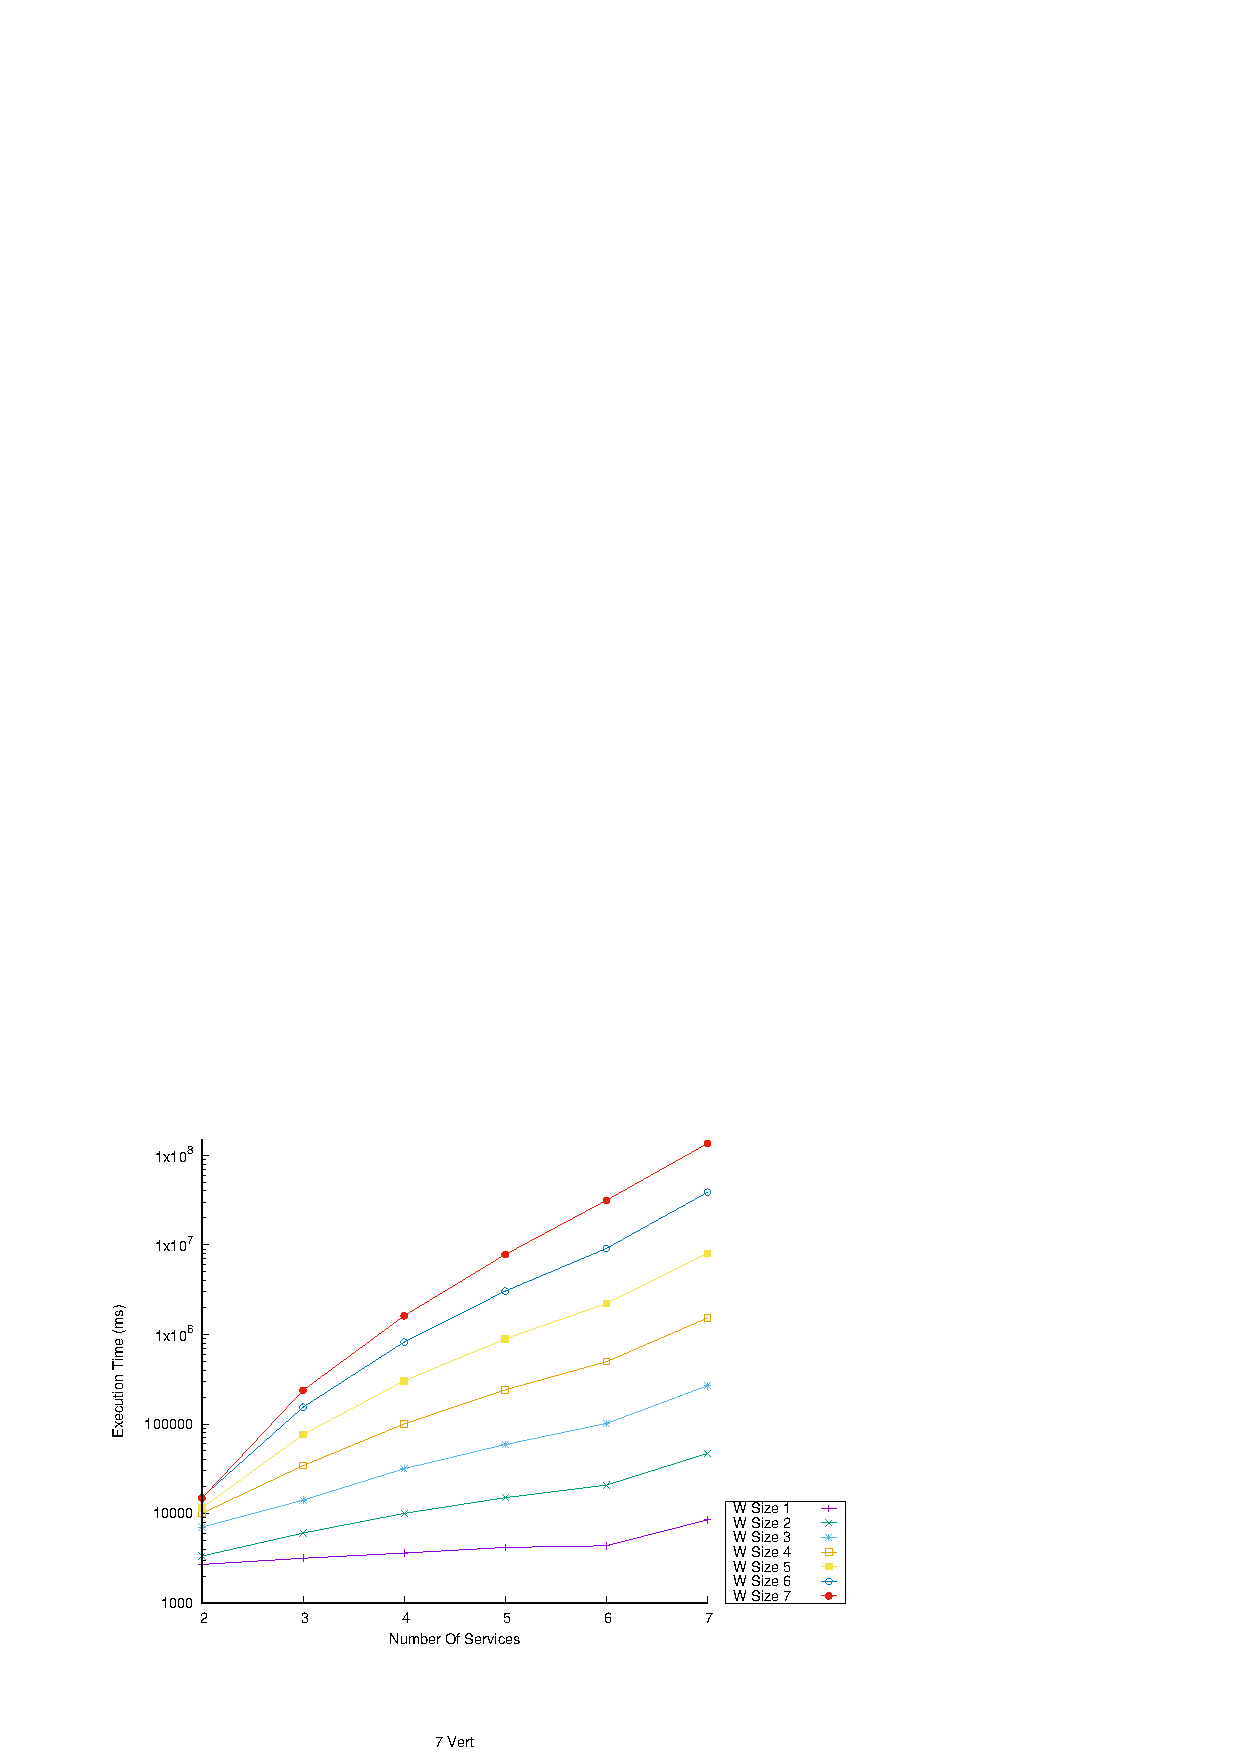
\includegraphics[width=\textwidth]{Images/graphs/window_time_performance_qualitative_n7_s7_50_80_n7}
      \caption{7 vertices}
      \label{fig:time_window_perce_wide_7n}
    \end{subfigure}
    \label{fig:time_window_perce_average}
  \end{figure}
  %   % \hfill
  %   % \begin{subfigure}{0.33\textwidth}
  %   %   \includegraphics[width=\textwidth]{Images/graphs/quality_plot_average_n7.eps}
  %   %   \caption{7 vertices}
  %   %   \label{fig:third}
  %   % \end{subfigure}
  %   \caption{Evaluation of Execution Time Using the \emph{Qaulitative} Metric in a \average Profile Configuration.}  \label{fig:time_window_perce_wide}
  % \end{figure}
  % \begin{figure}[!htb]
  %   \centering
  %   \begin{subfigure}{0.45\textwidth}
  %     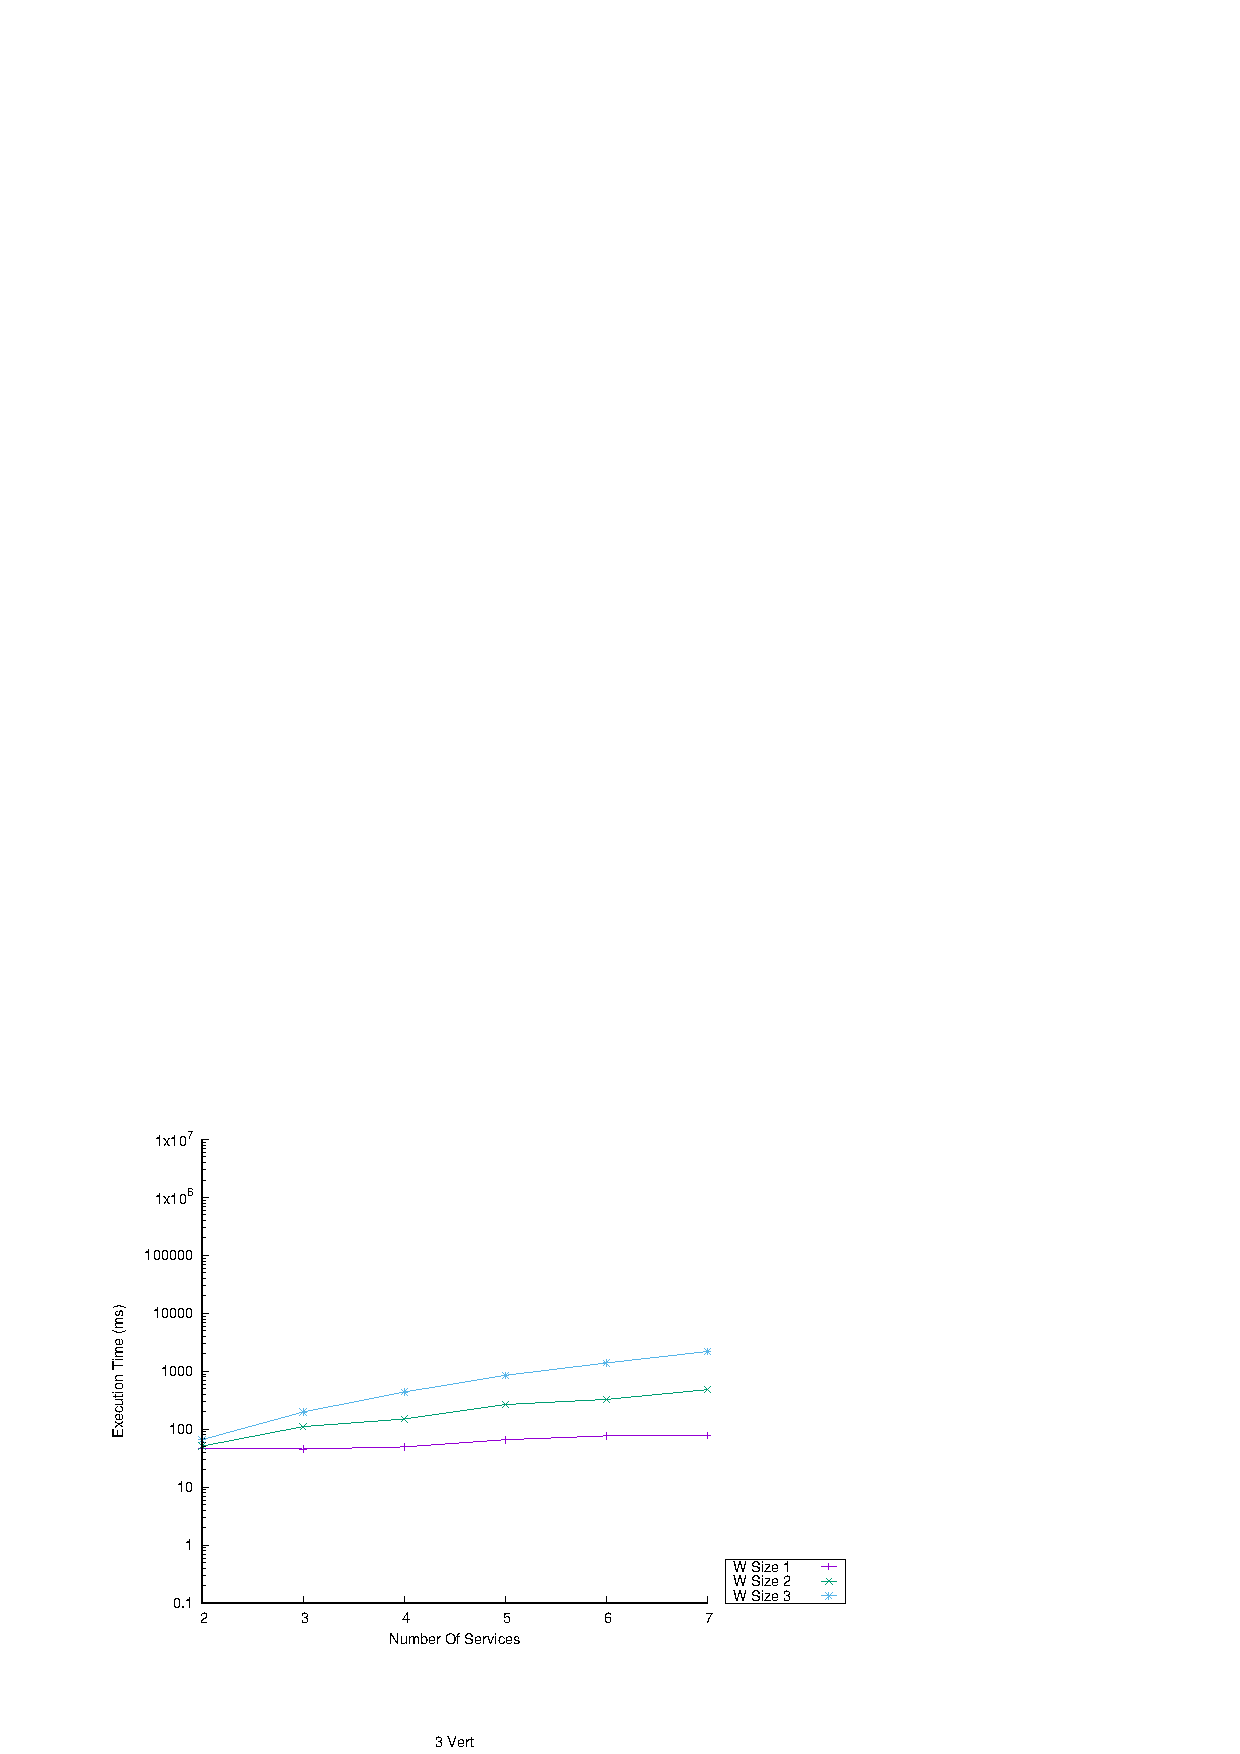
\includegraphics[width=\textwidth]{Images/graphs/window_time_performance_n7_s7_20_100_n3}
  %     \caption{3 vertices}
  %     \label{fig:time_window_perce_average_3n}
  %   \end{subfigure}
  %   \hfill
  %   \begin{subfigure}{0.45\textwidth}
  %     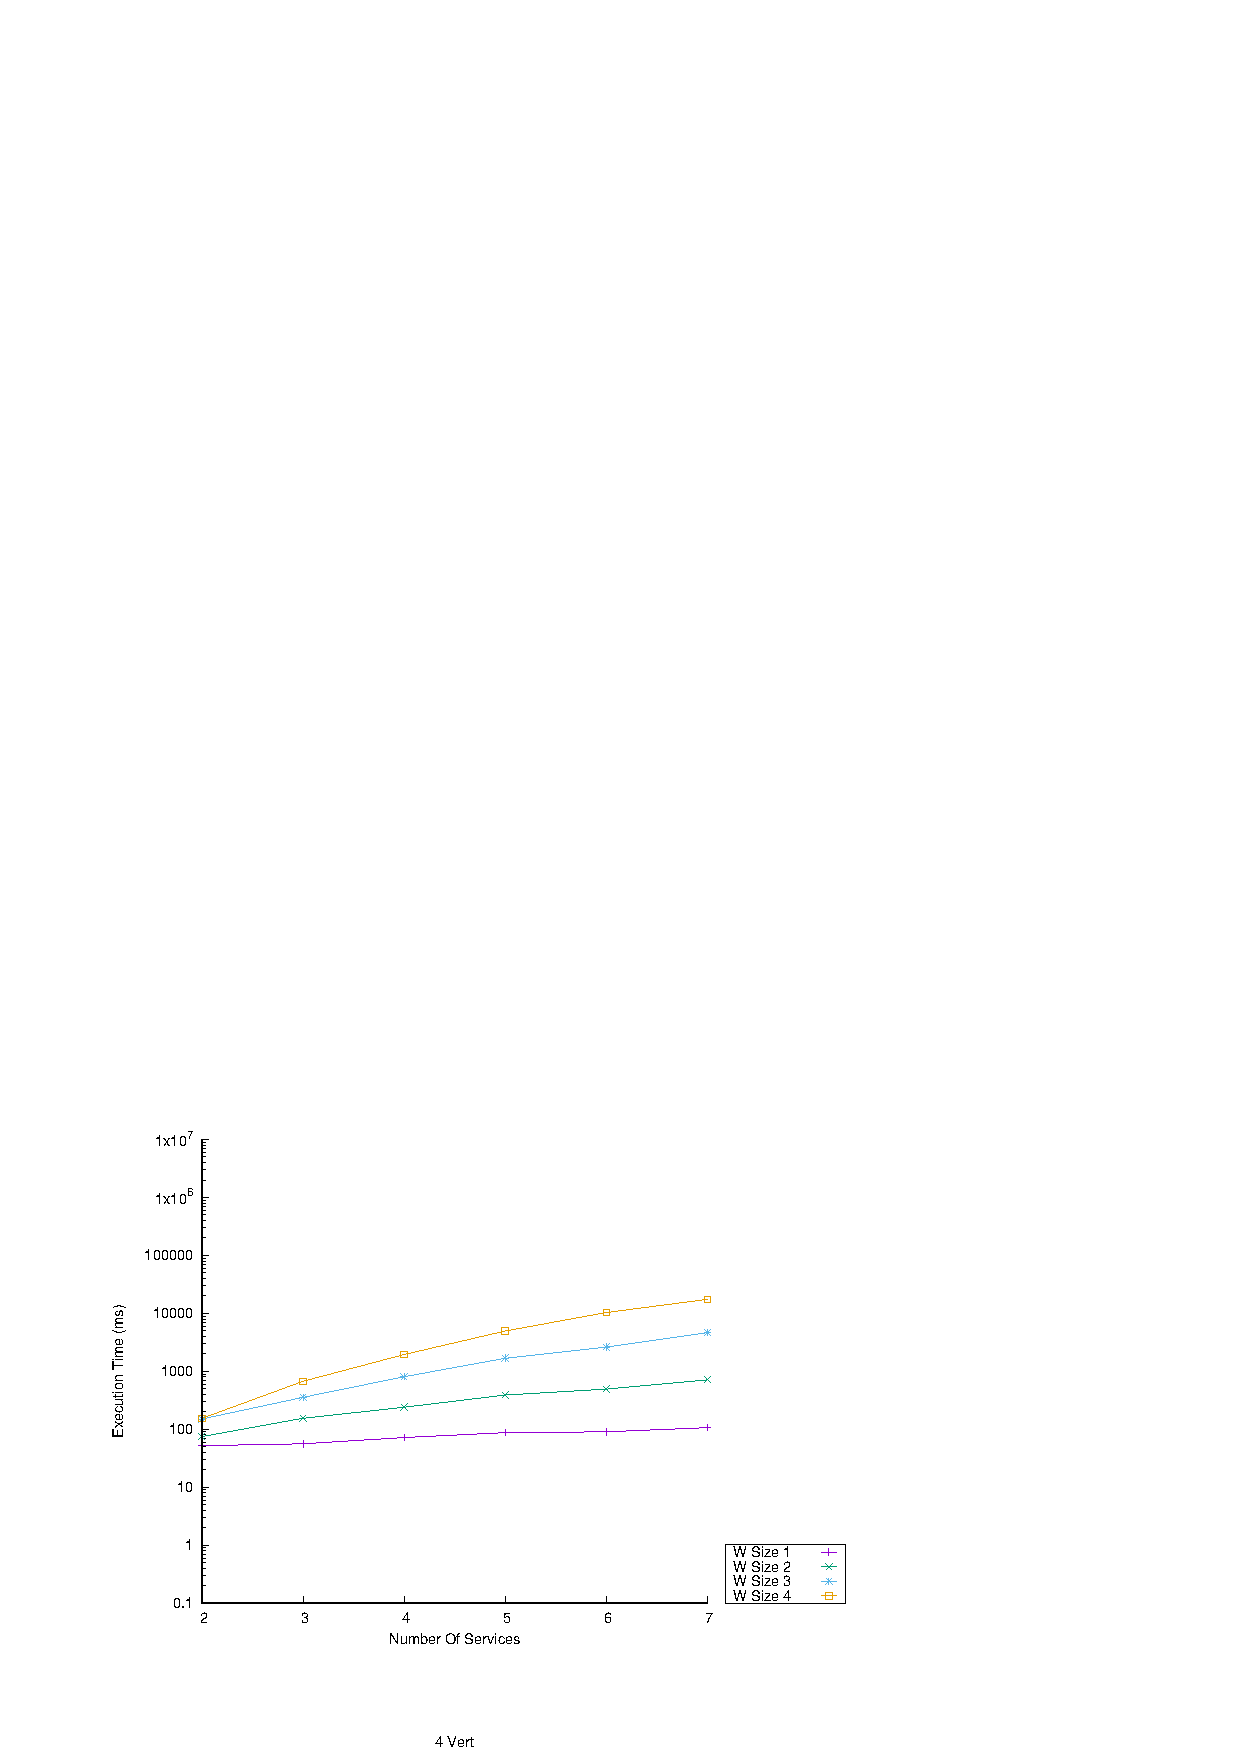
\includegraphics[width=\textwidth]{Images/graphs/window_time_performance_n7_s7_20_100_n4}
  %     \caption{4 vertices}
  %     \label{fig:time_window_perce_average_4n}
  %   \end{subfigure}
  %   \hfill
  %   \begin{subfigure}{0.45\textwidth}
  %     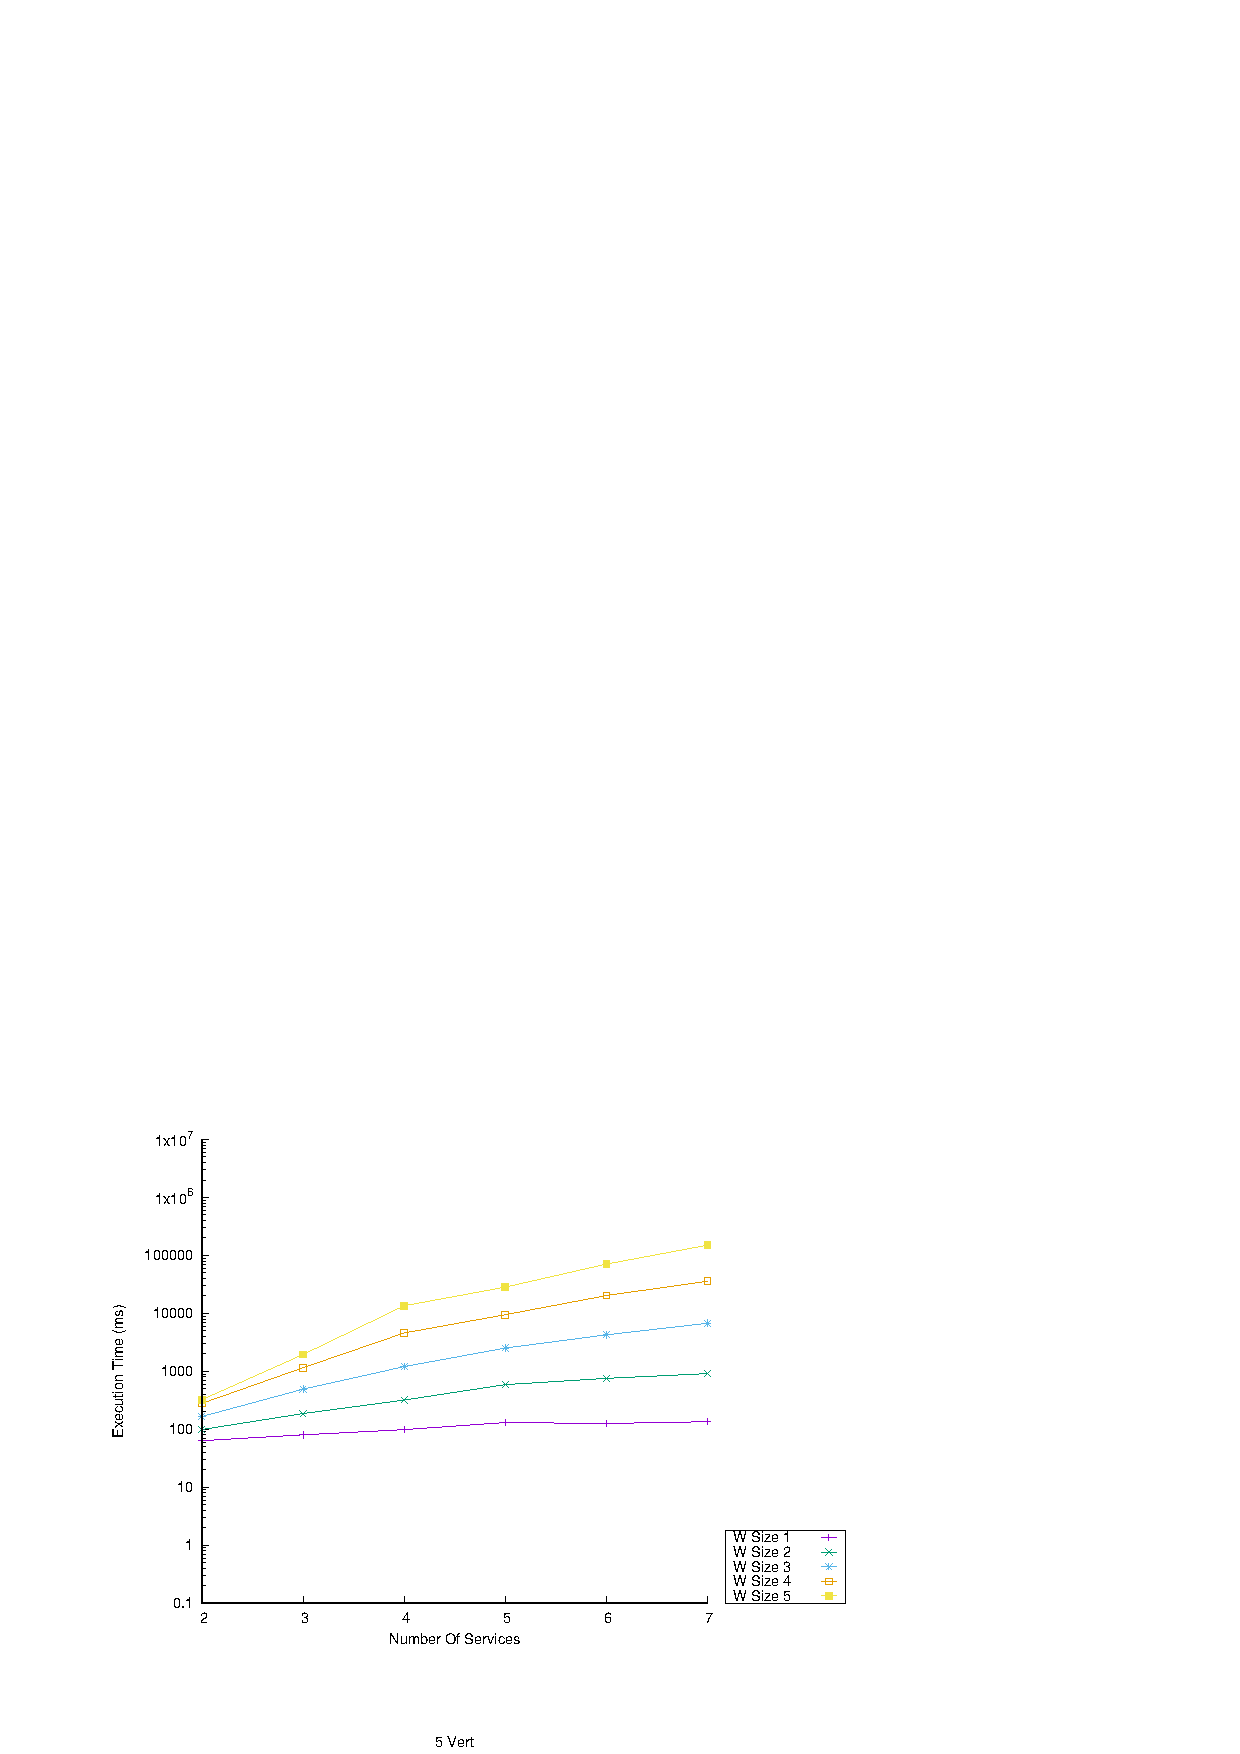
\includegraphics[width=\textwidth]{Images/graphs/window_time_performance_n7_s7_20_100_n5}
  %     \caption{5 vertices}
  %     \label{fig:time_window_perce_average_5n}
  %   \end{subfigure}
  %   \hfill
  %   \begin{subfigure}{0.45\textwidth}
  %     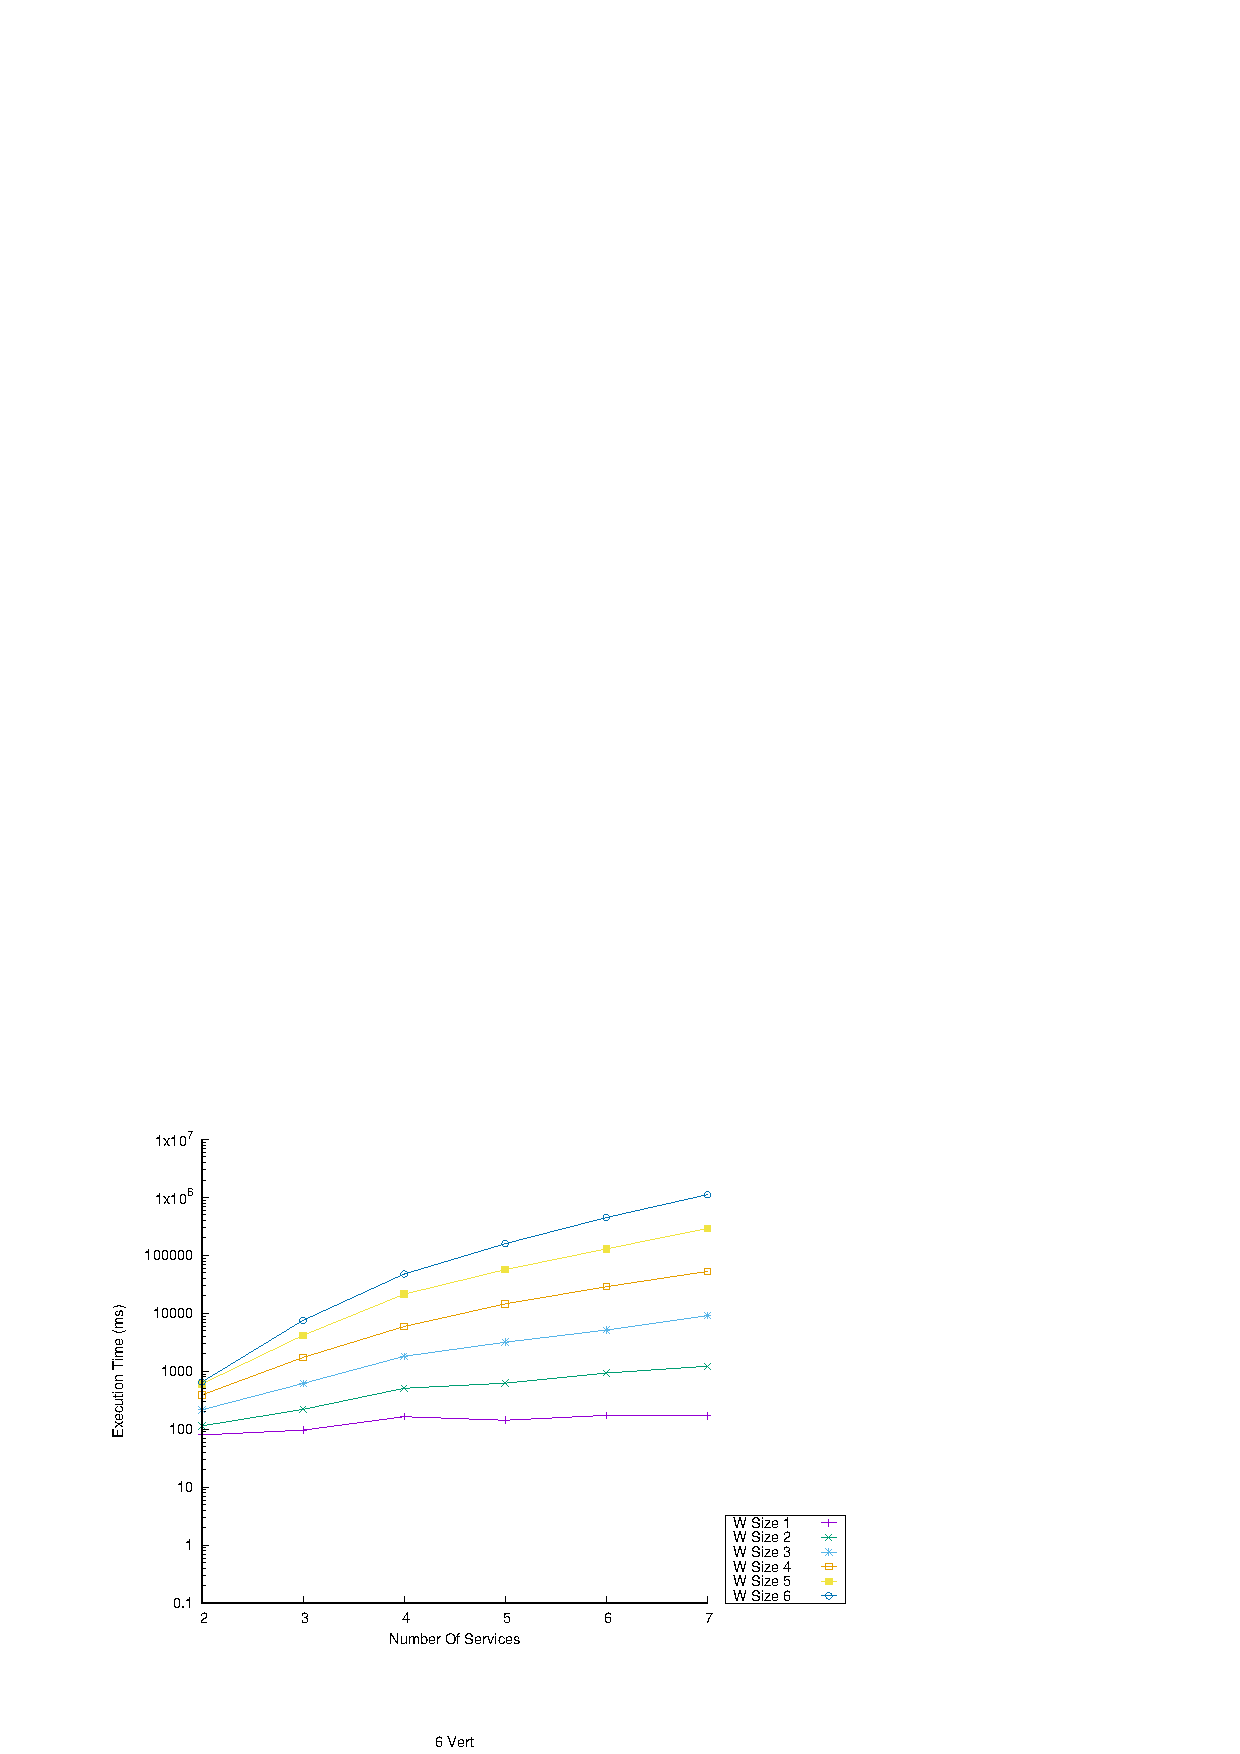
\includegraphics[width=\textwidth]{Images/graphs/window_time_performance_n7_s7_20_100_n6}
  %     \caption{6 vertices}
  %     \label{fig:time_window_perce_average_6n}
  %   \end{subfigure}
  %   \begin{subfigure}{0.45\textwidth}
  %     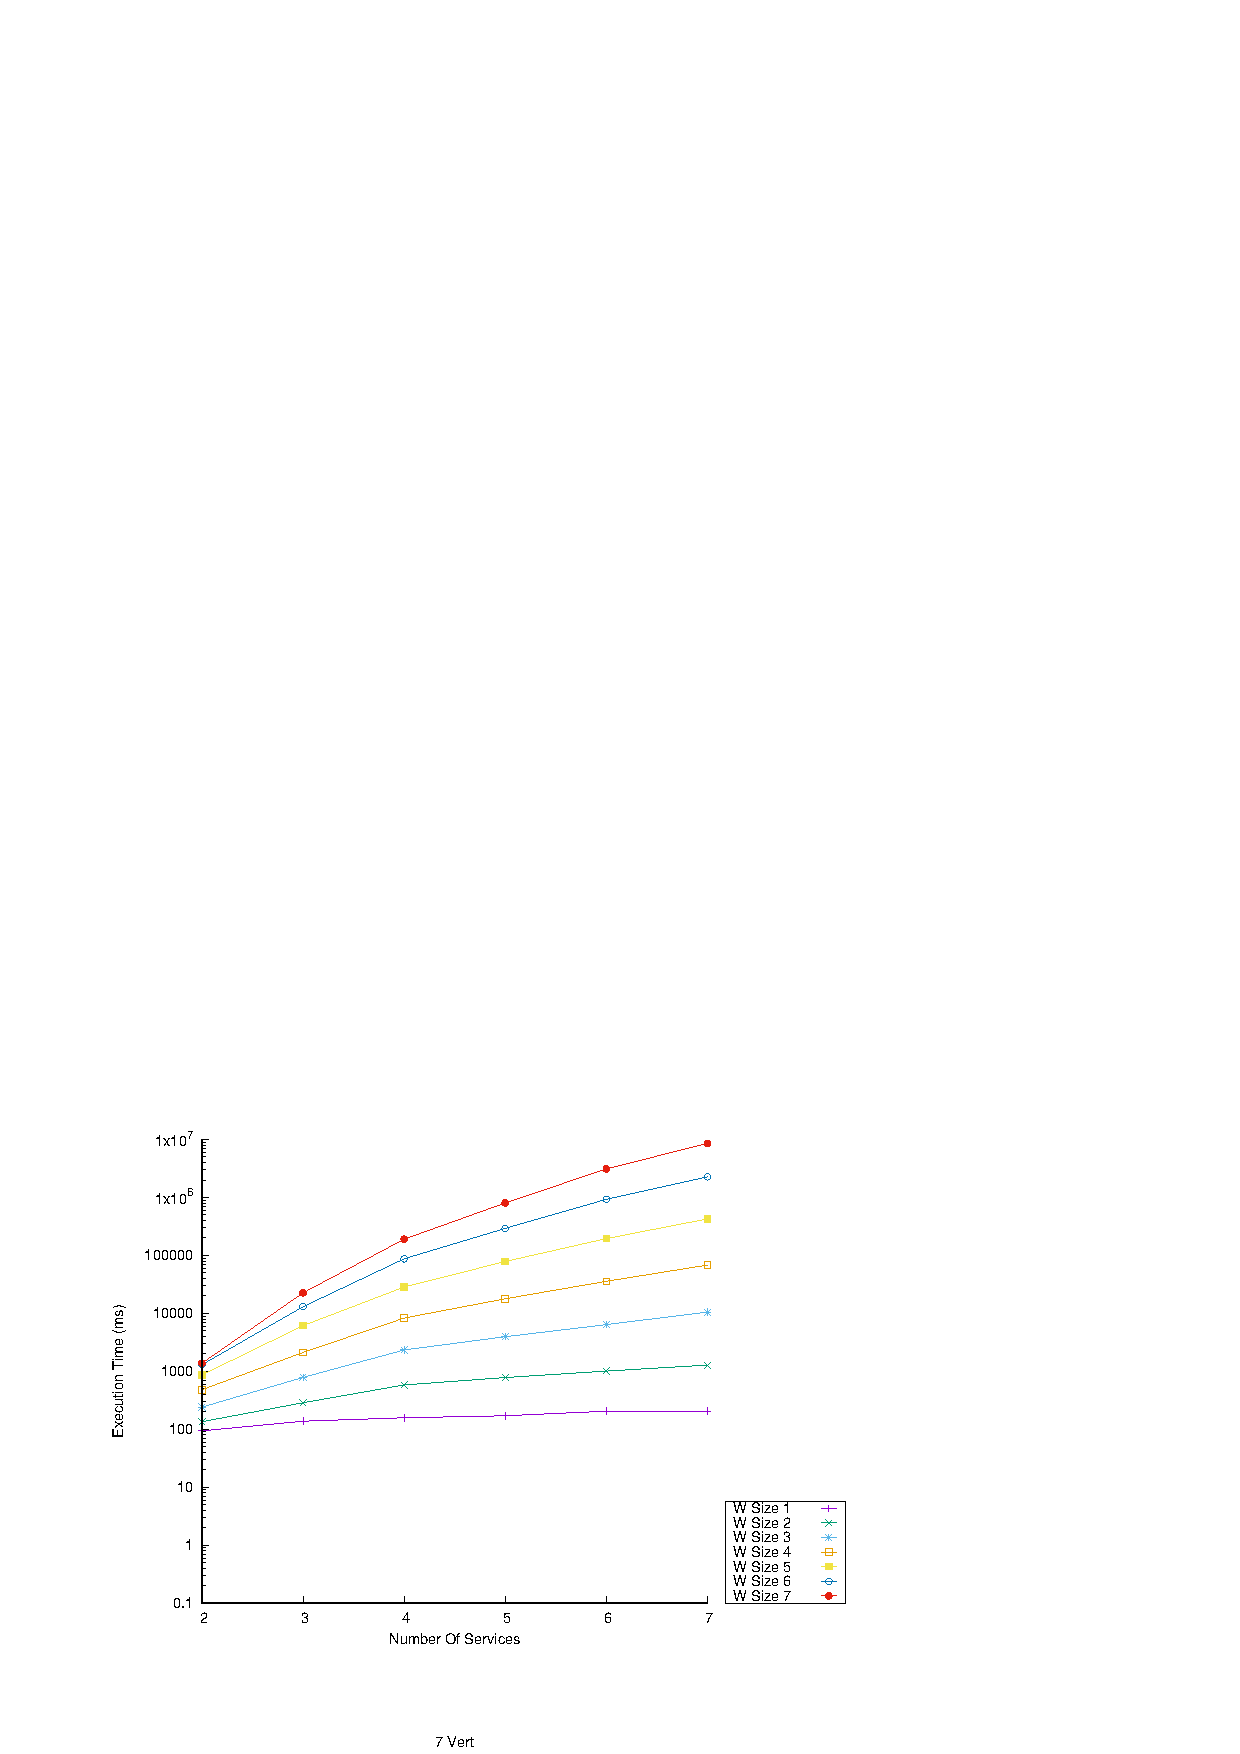
\includegraphics[width=\textwidth]{Images/graphs/window_time_performance_n7_s7_20_100_n7}
  %     \caption{7 vertices}
  %     \label{fig:time_window_perce_average_7n}polo
  %   \end{subfigure}
  %   % \hfill
  %   % \begin{subfigure}{0.33\textwidth}
  %   %   \includegraphics[width=\textwidth]{Images/graphs/quality_plot_average_n7.eps}
  %   %   \caption{7 vertices}
  %   %   \label{fig:third}
  %   % \end{subfigure}
  %   \caption{Evaluation of Execution Time Using the \emph{Quantitative} Metric in a \average Profile Configuration.}

  \subsection{Quality}\label{subsec:experiments_quality}
  We finally evaluated the quality of our heuristic algorithm with different \windowsize\ comparing, where possible, its results with the optimal solution retrieved by executing the exhaustive approach. %The latter is executed with window size equals to the number of vertices in the pipeline template, and provides the best, among all possible, solutions.
  The quality $Q$ of the heuristic has been normalized between 0 and 1 by dividing it by the quality $Q*$ retrieved by the exhaustive approach.


  We run our experiments varying: \emph{i)} the length $l$ of the pipeline template in [3,7], that is, the number of vertices composed in a sequence, \emph{ii)} the window size \windowsize\ in [1,$l$], and \emph{iii)} the number of candidate services for each vertex in the pipeline template in [2, 7]. Each vertex is associated with a (set of) policy that applies a filtering transformation that either remove a percentage of data in $[0.5,0.8]$ (\average) or in $[0.20,1]$ (\wide).

  \cref{fig:quality_window_perce} present our quality results using metric $M_J$ in \cref{subsec:metrics} for settings \wide and \average.
  In general, we observe that the quality of our heuristic approach increases as the window size increases, providing a quality comparable to the exhaustive approach when the window size \windowsize\ approaches the length $l$ of the pipeline template.

  When considering setting \wide, the greedy approach (\windowsize=1) provides good results on average (0.71, 0.90), while showing substantial quality oscillations in specific runs: between 0.882 and 0.970 for 3 vertices, 0.810 and 0.942 for 4 vertices, 0.580 and 0.853 for 5 vertices, 0.682 and 0.943 for 6 vertices, 0.596 and 0.821 for 7 vertices. This same trend emerges when the window size is $<$$l$/2, while it starts approaching the optimum when the window size is $\geq$$l$/2. For instance, when \windowsize=$l$-1, the quality varies between 0.957 and 1.0 for 3 vertices, 0.982 and 1.0 for 4 vertices, 0.986 and 0.998 for 5 vertices, 0.977 and 1.0 for 6 vertices, 0.996 and 1.0 for 7 vertices.

  When considering setting \average, the heuristic algorithm still provides good results, limiting the quality oscillations observed for setting \wide\ and approaching the quality of the exhaustive also for lower window sizes. The greedy approach (\windowsize=1) provides good results on average (from 0.842 to 0.944), as well as in specific runs: between 0.927 and 0.978 for 3 vertices, 0.903 and 0.962 for 4 vertices, 0.840 and 0.915 for 5 vertices, 0.815 and 0.934 for 6 vertices, 0.721 and 0.935 for 7 vertices.
  %This same trend emerges when the window size is less than $l$/2, while it starts approaching the optimum when the window size is higher than $l$/2. For instance,
  When \windowsize=$l$-1, the quality varies between 0.980 and 1.0 for 3 vertices, 0.978 and 1.0 for 4 vertices, 0.954 and 1 for 5 vertices, 0.987 and 1.0 for 6 vertices, 0.990 and 1.0 for 7 vertices.


  \cref{fig:quality_window_qualitative} present our quality results using metric $M_{JSD}$ in \cref{subsec:metrics} for settings \wide and \average, respectively.
  % In general, \hl{ANTONGIACOMO}

  When considering setting \wide, the greedy approach (\windowsize=1) provides good results on average (0.92, 0.97), it shows substantial oscillations, for instance, varying the quality between 0.951 and 0.989 for 3 vertices, 0.941 and 0.988 for 4 vertices, 0.919 and 0.974 for 5 vertices, 0.911 and 0.971 for 6 vertices, 0.877 and 0.924 for 7 vertices. In this case the quality oscillations are more stable than the ones observed for the metric $M_J$.
  In general the worst quality is obtained with window size equal to 1, while the oscillations reduces as the window size is >2. For instance, when \windowsize=$l$-2, the quality varies between, 0.982 and 0.996 for 4 vertices, 0.981 and 0.998 for 5 vertices, 0.988 and 1.0 for 6 vertices, 0.976 and 0.999 for 7 vertices.
 While, when \windowsize=$l$-1, the quality varis between  0.987 and  0.998 for 3 vertices, 0.993 and 1.0 for 4 vertices, 0.985 and 0.999 for 5 vertices, 0.997 and 1.0 for 6 vertices, 0.995 and 1.0  for 7 vertices.


  When considering setting \average, the greedy approach (\windowsize=1) provides good results on average (from 0.920 to 0.969), it shows substantial oscillations, for instance, varying the quality between 0.951 and 0.989 for 3 vertices, 0.942 and 0.988 for 4 vertices, 0.919 and 0.975 for 5 vertices, 0.912 and 0.972 for 6 vertices, 0.878 and 0.925 for 7 vertices. The \average configuration provides even tighter quality oscillations than the \wide configuration. In general the worst quality is obtained with window size equal to 1, while the oscillations reduces as the \windowsize is $>1$ (e.g. $v=3$,$v=4$) or $>2$ (e.g. $v=5$,$v=6$,$v=7$).

  For instance, when \windowsize=3, the quality varis between  0.993 and 1 for 4 vertices, 0.981 and 0.998 for 5 vertices, 0.982 and 997 for 6 vertices, 0.960 and 0.991 for 7 vertices.


  Our results suggest that the proposed heuristic well approximates the results obtained via an exhaustive approach. While larger window sizes generally lead to better performance, there exists a point where the balance between window size and performance is optimized. Beyond this point, the incremental gains in metric values may not justify the additional computational burden or complexity introduced by larger windows. It is worth noting that lower window sizes are more unstable, especially with setting \wide, meaning that the quality varies significantly among different configurations. This effect stabilizes with higher window sizes (e.g., \windowsize$\geq$$l$/2).

\begin{figure}[H]
  \centering
  \begin{subfigure}{0.45\textwidth}
    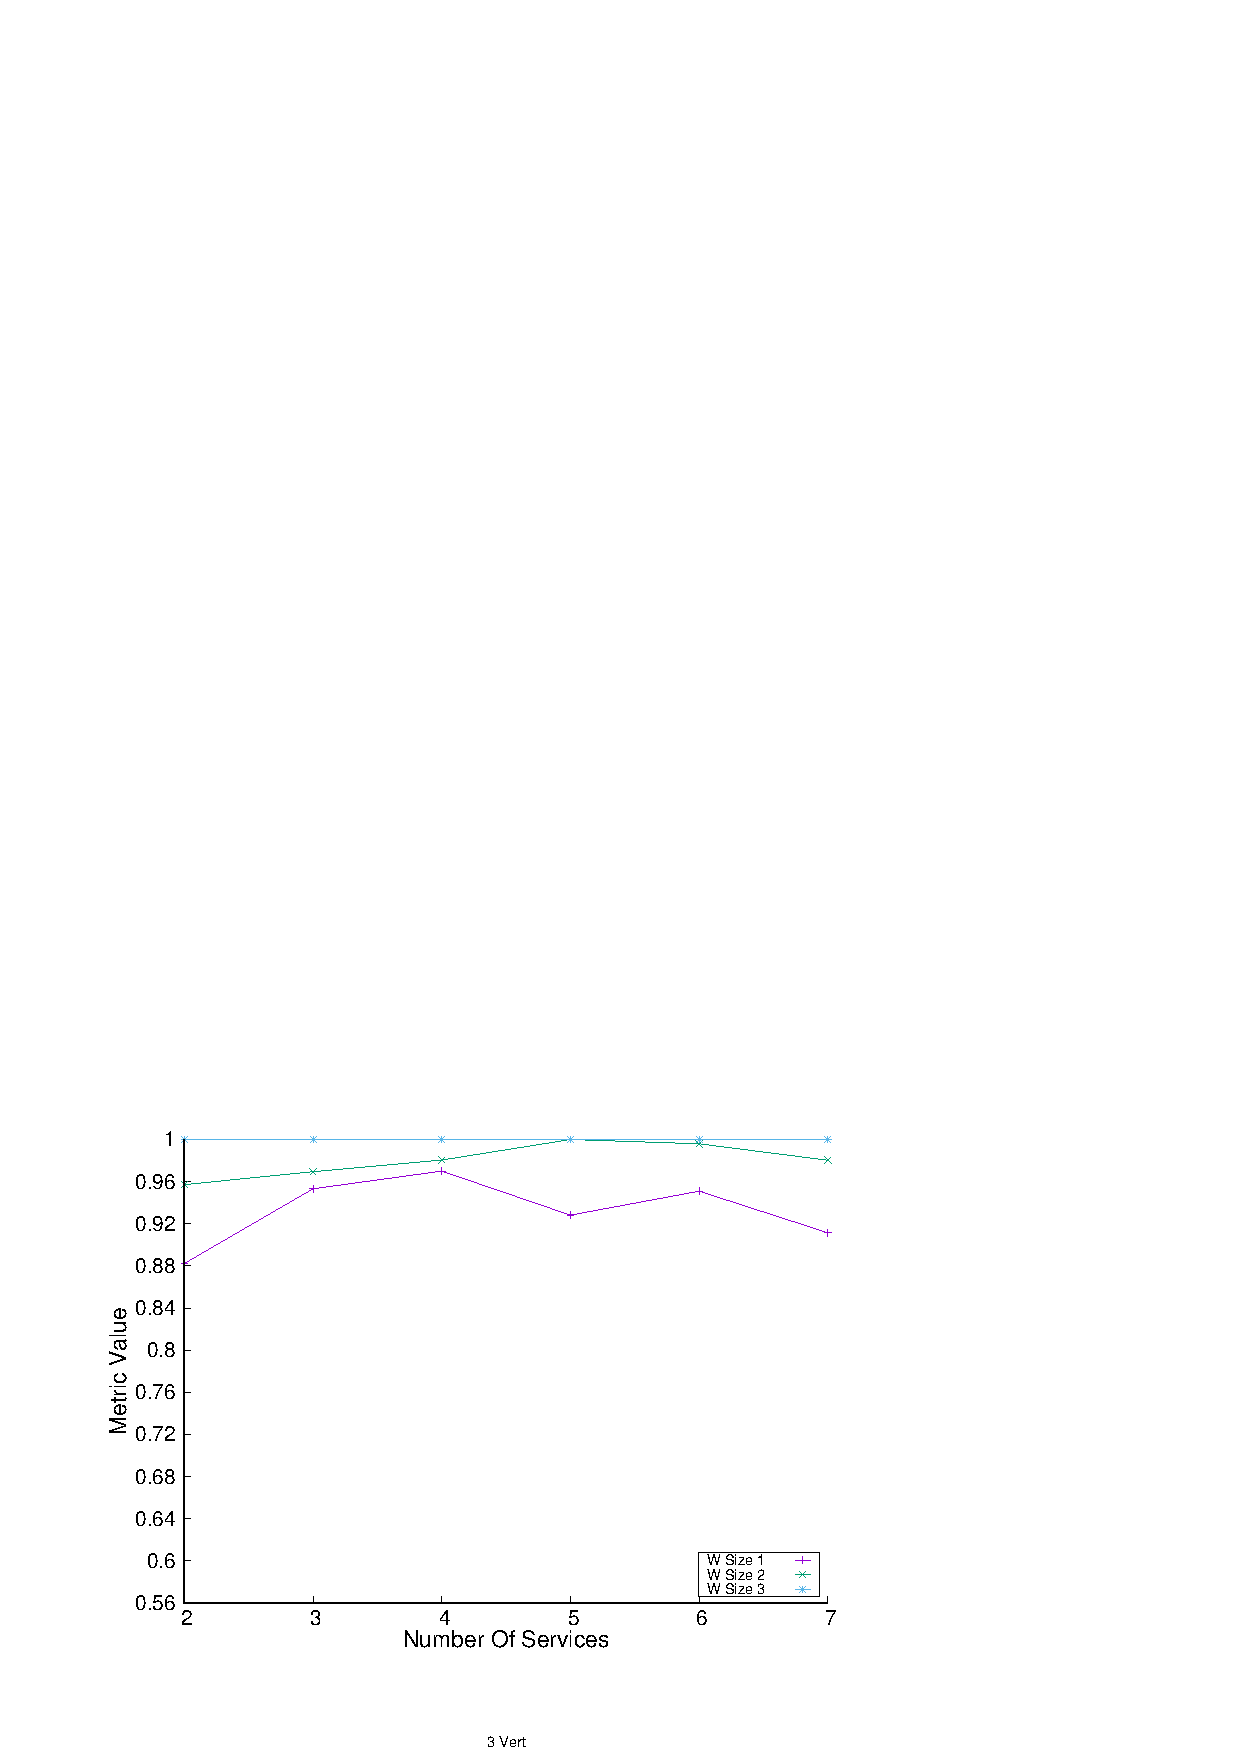
\includegraphics[width=\textwidth]{Images/graphs/window_quality_performance_diff_perce_n7_s7_20_100_n3}
    \caption{\wide 3 vertices}
    \label{fig:quality_window_perce_wide_3n}
  \end{subfigure}
  \hfill
  \begin{subfigure}{0.45\textwidth}
    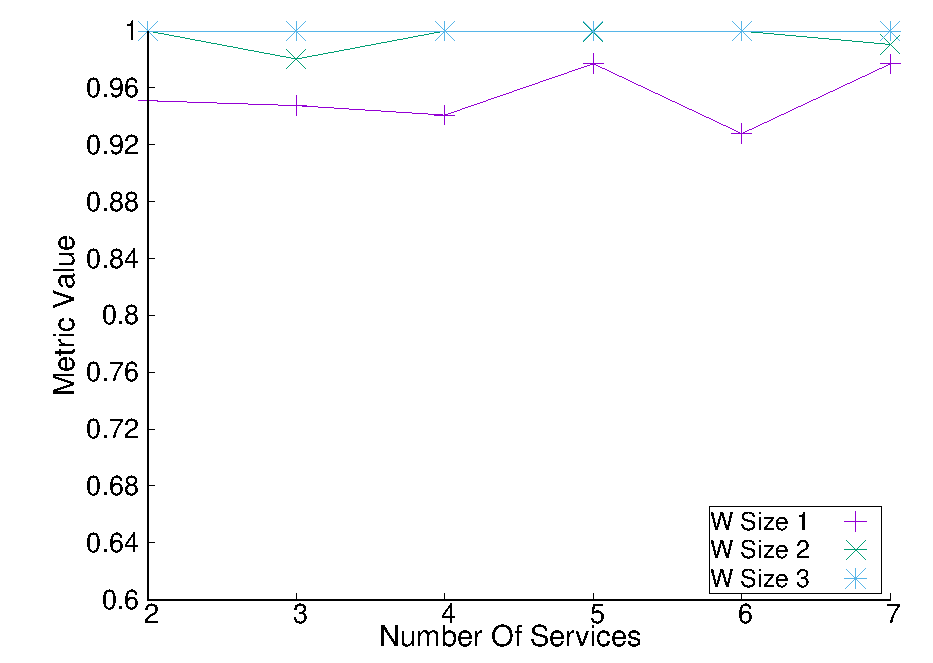
\includegraphics[width=\textwidth]{Images/graphs/window_quality_performance_diff_perce_n7_s7_50_89_n3}
    \caption{\average 3 vertices}
    \label{fig:quality_window_average_perce_3n}
  \end{subfigure}
  \begin{subfigure}{0.45\textwidth}
    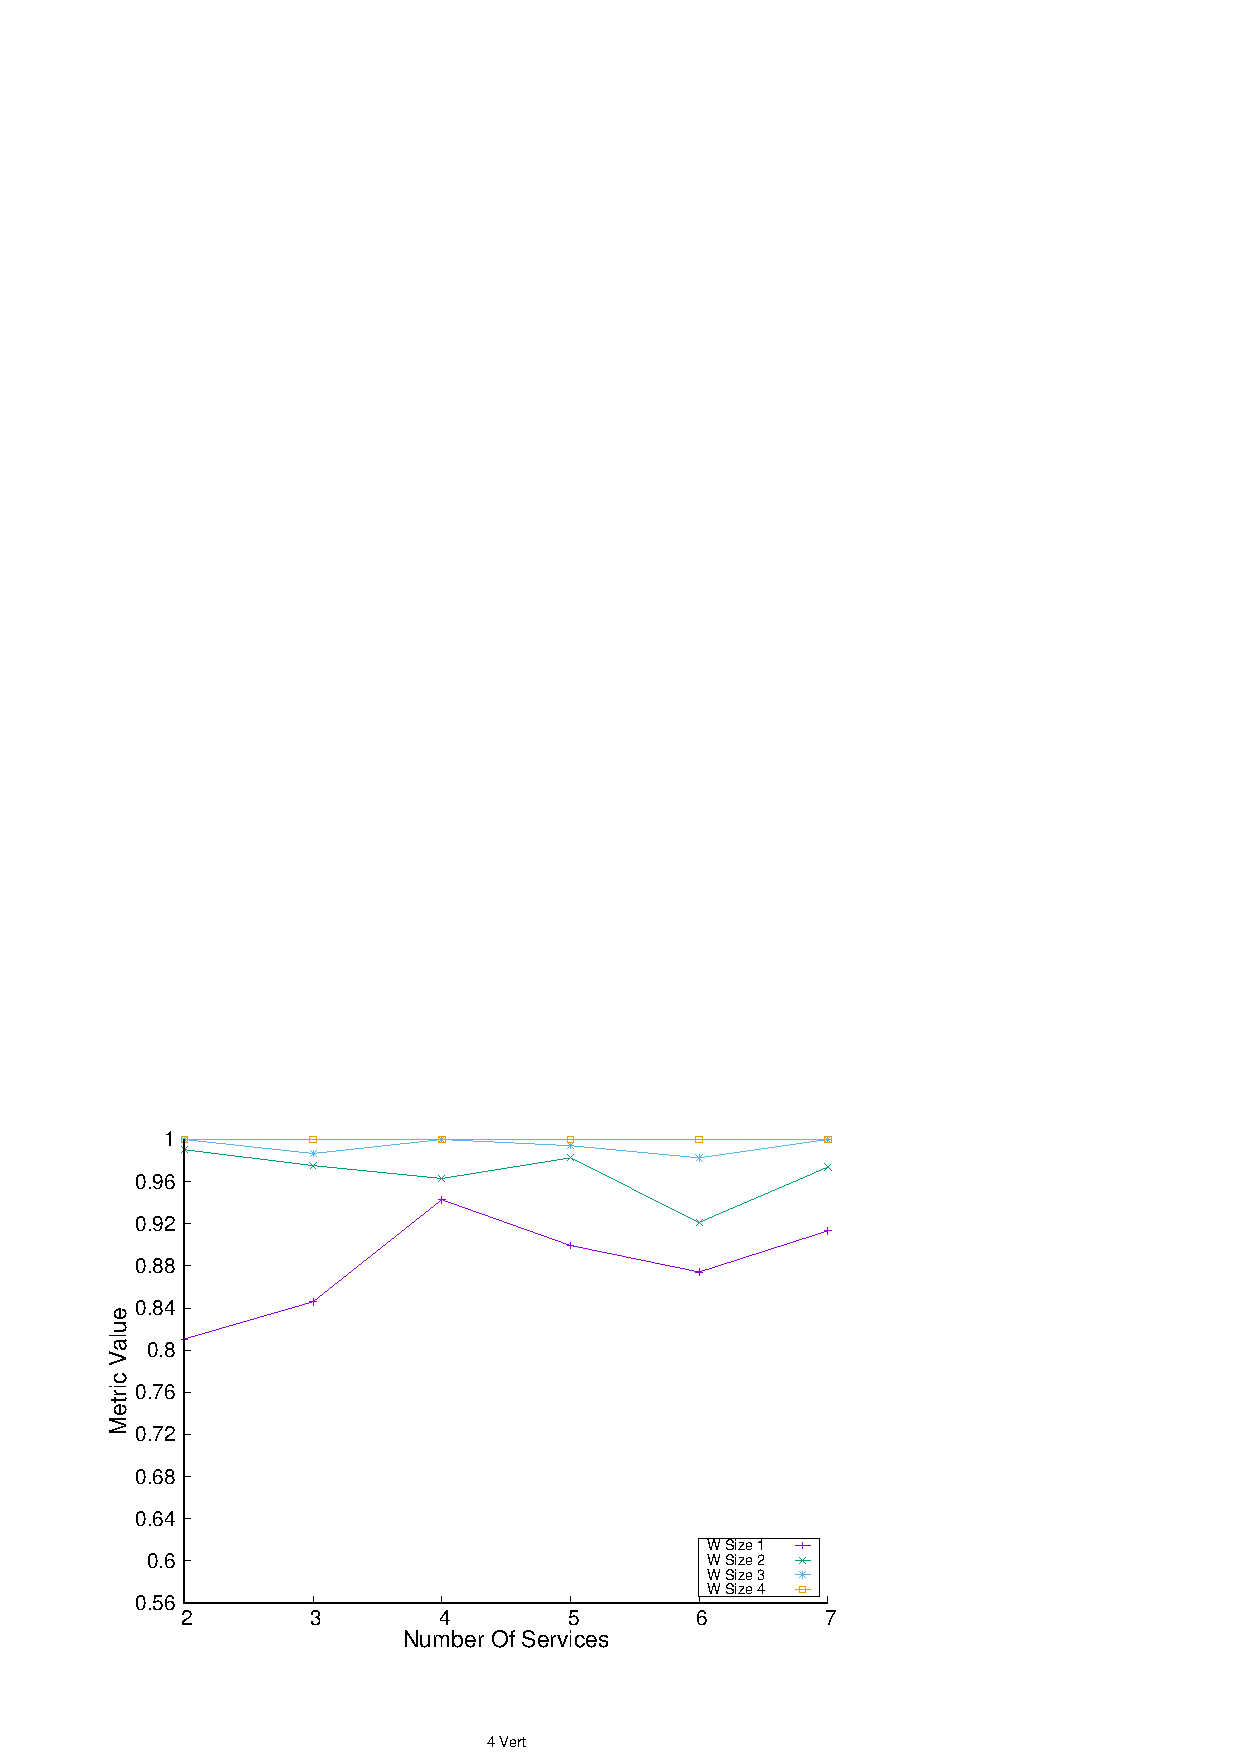
\includegraphics[width=\textwidth]{Images/graphs/window_quality_performance_diff_perce_n7_s7_20_100_n4}
    \caption{\wide 4 vertices}
    \label{fig:quality_window_perce_wide_4n}
  \end{subfigure}
  \hfill
  \begin{subfigure}{0.45\textwidth}
    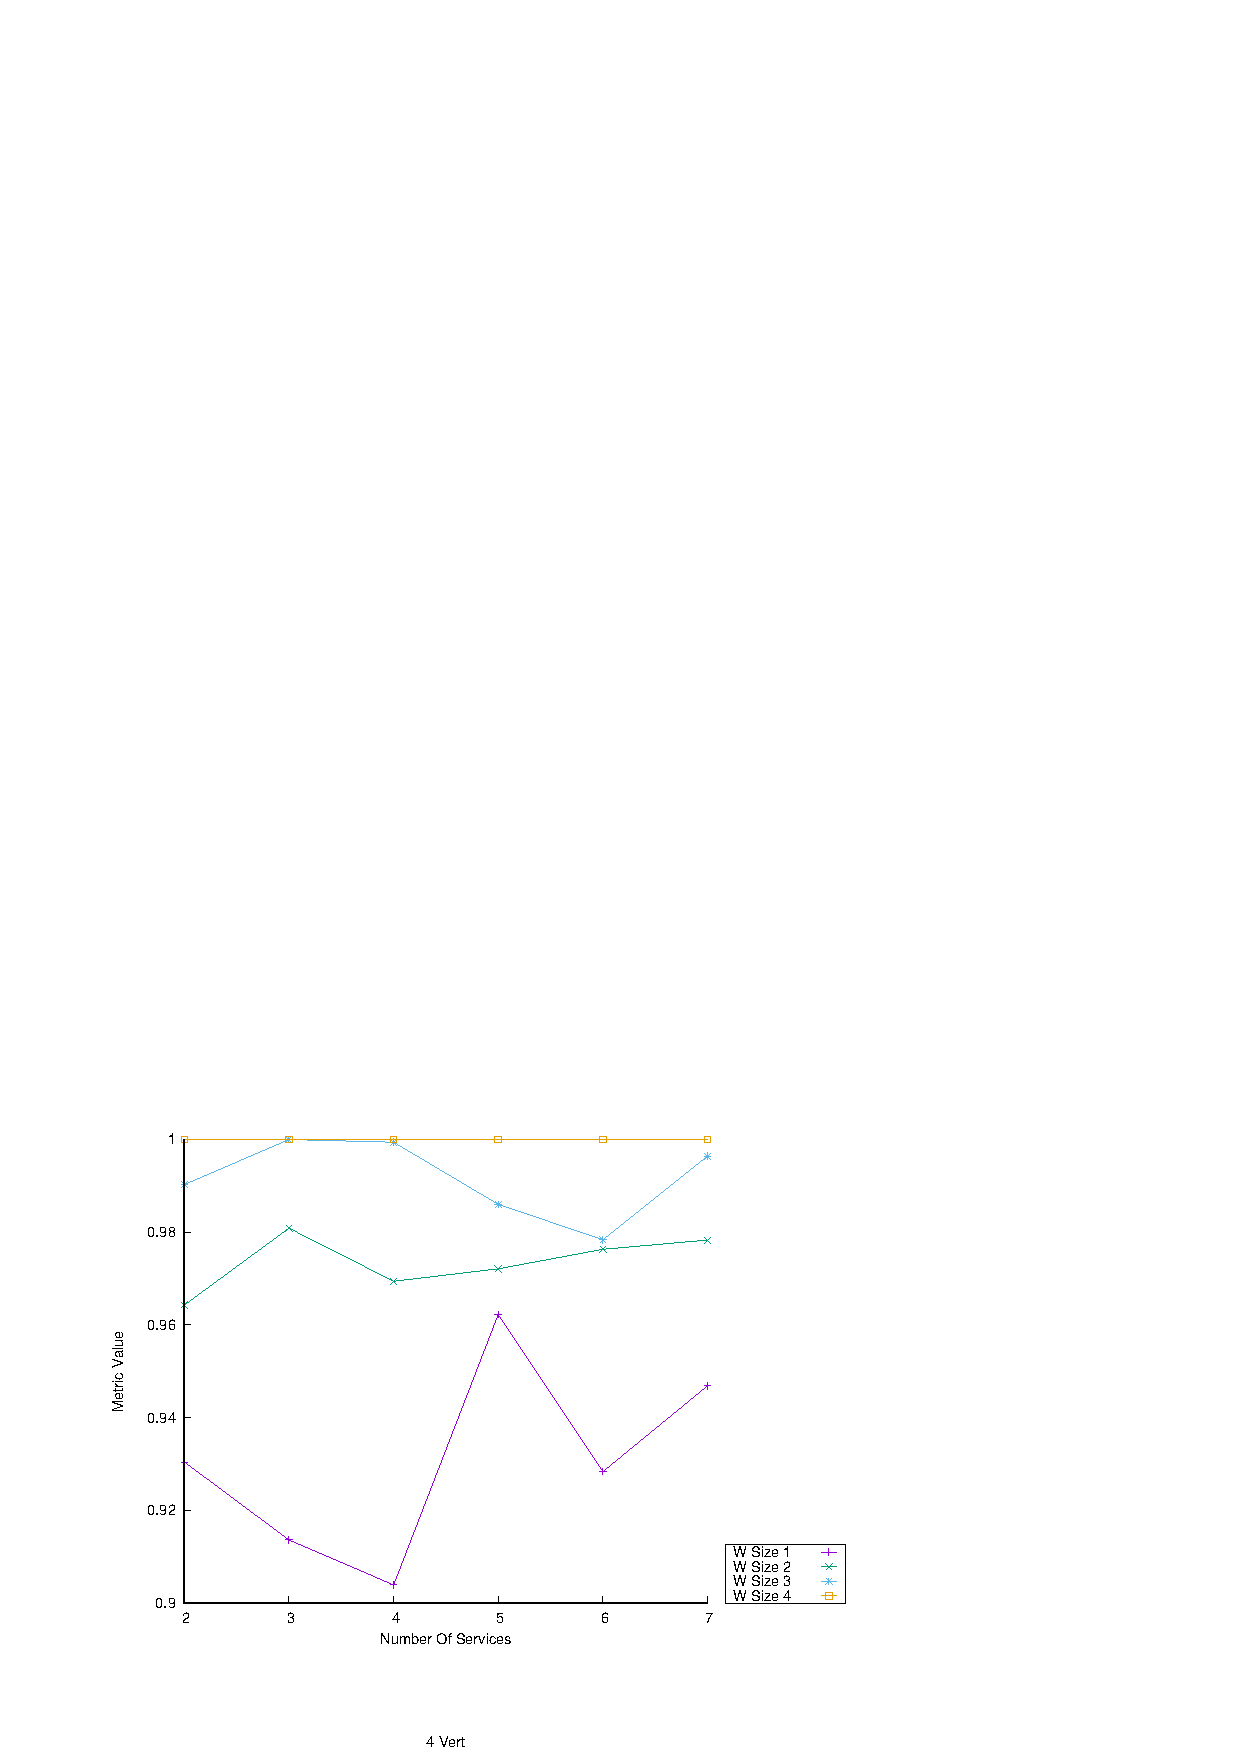
\includegraphics[width=\textwidth]{Images/graphs/window_quality_performance_diff_perce_n7_s7_50_89_n4}
    \caption{\average 4 vertices}
    \label{fig:quality_window_average_perce_4n}
  \end{subfigure}
  \hfill
  \begin{subfigure}{0.45\textwidth}
    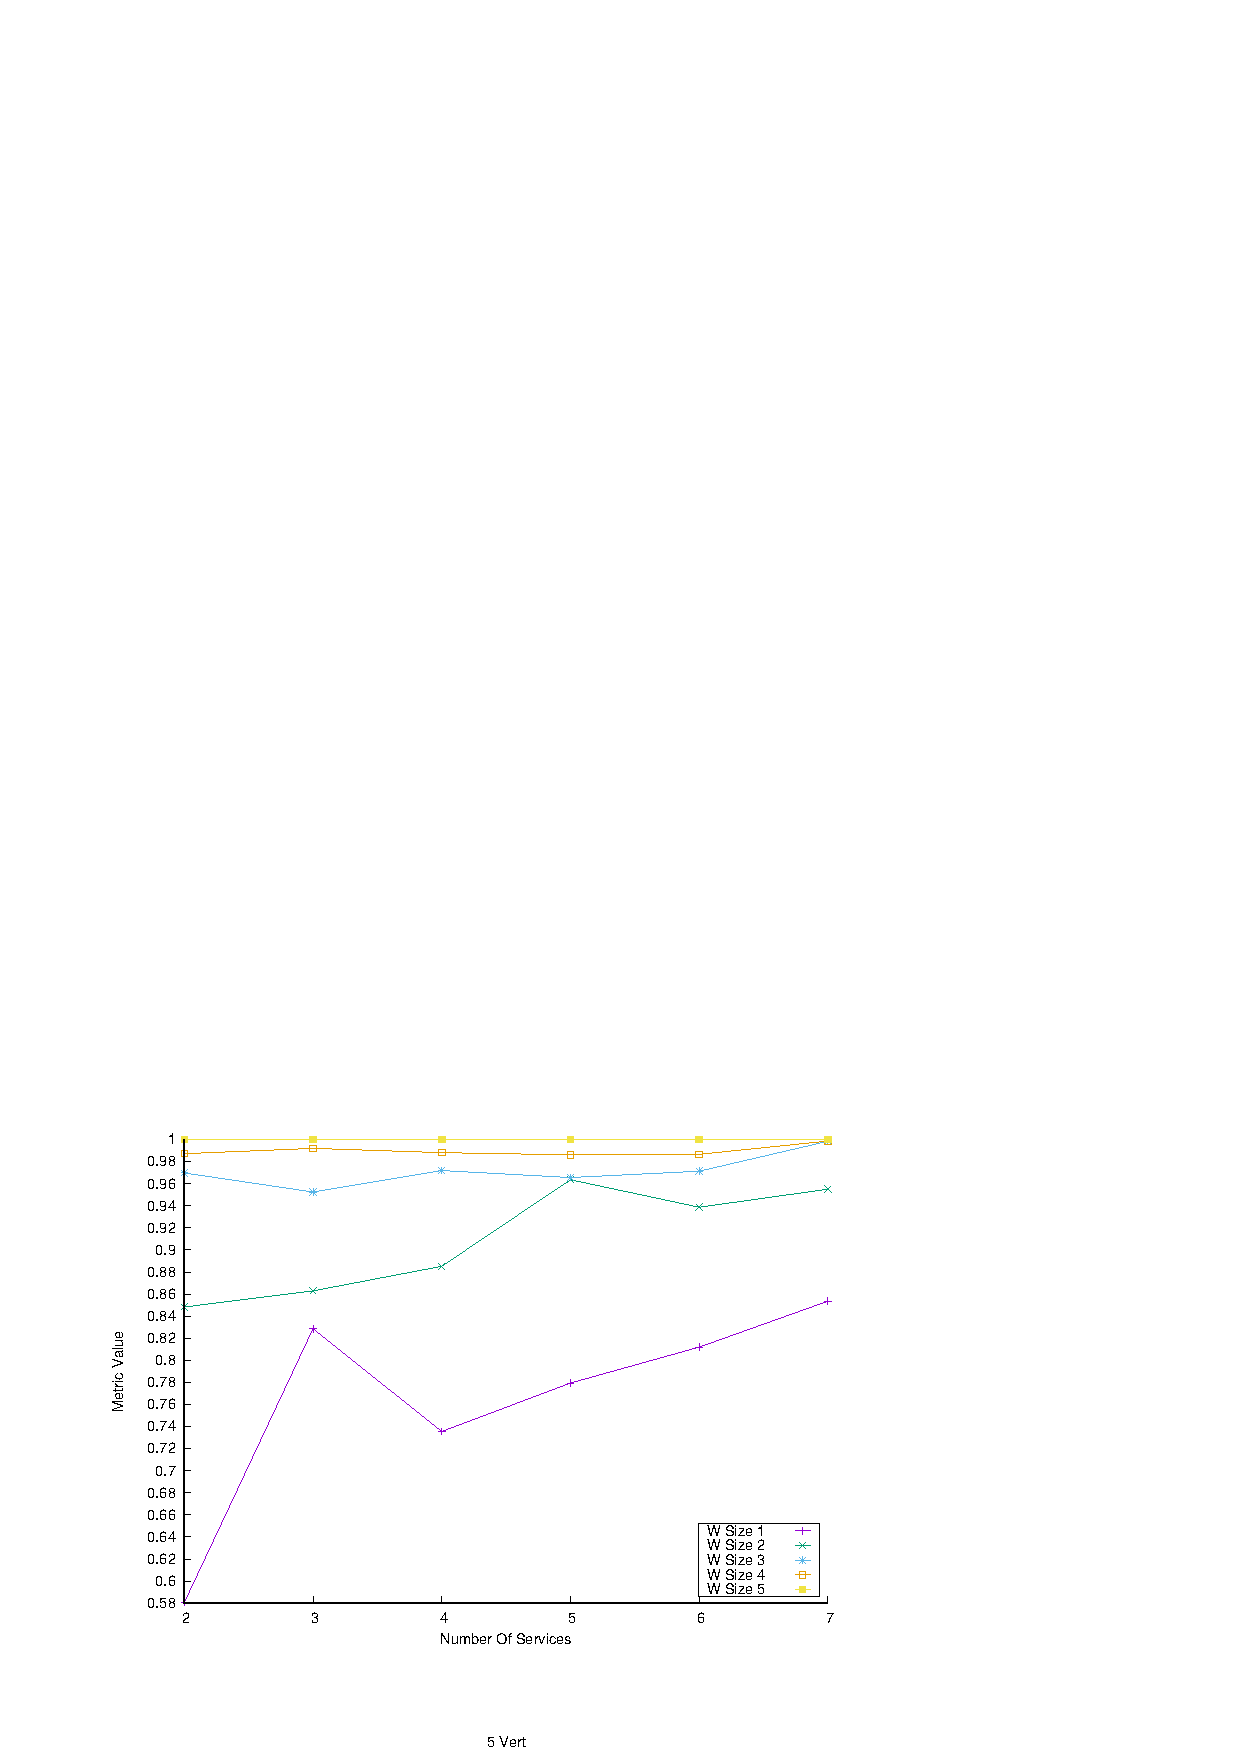
\includegraphics[width=\textwidth]{Images/graphs/window_quality_performance_diff_perce_n7_s7_20_100_n5}
    \caption{\wide 5 vertices}
    \label{fig:quality_window_perce_wide_5n}
  \end{subfigure}
  \hfill
  \begin{subfigure}{0.45\textwidth}
    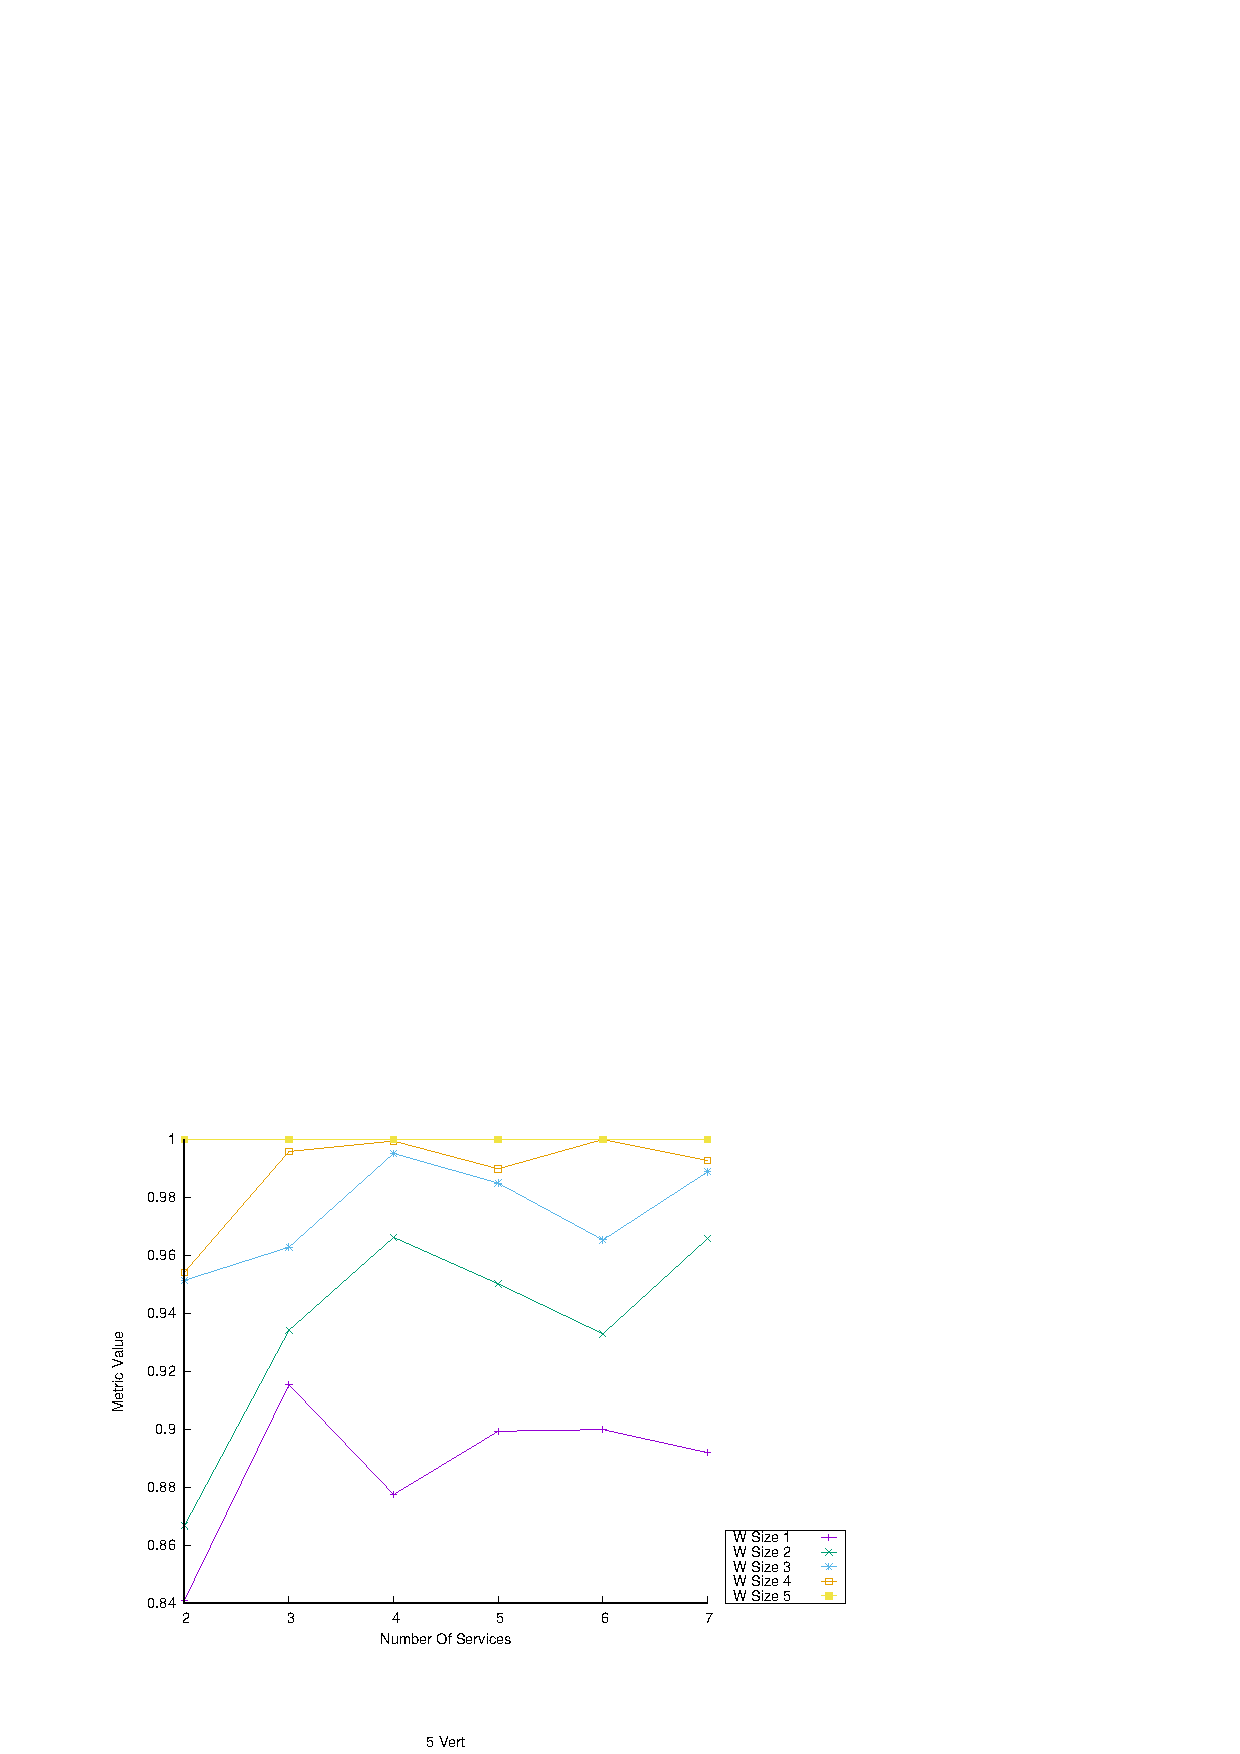
\includegraphics[width=\textwidth]{Images/graphs/window_quality_performance_diff_perce_n7_s7_50_89_n5}
    \caption{\average 5 vertices}
    \label{fig:quality_window_average_perce_5n}
  \end{subfigure}
  \hfill
  \begin{subfigure}{0.45\textwidth}
    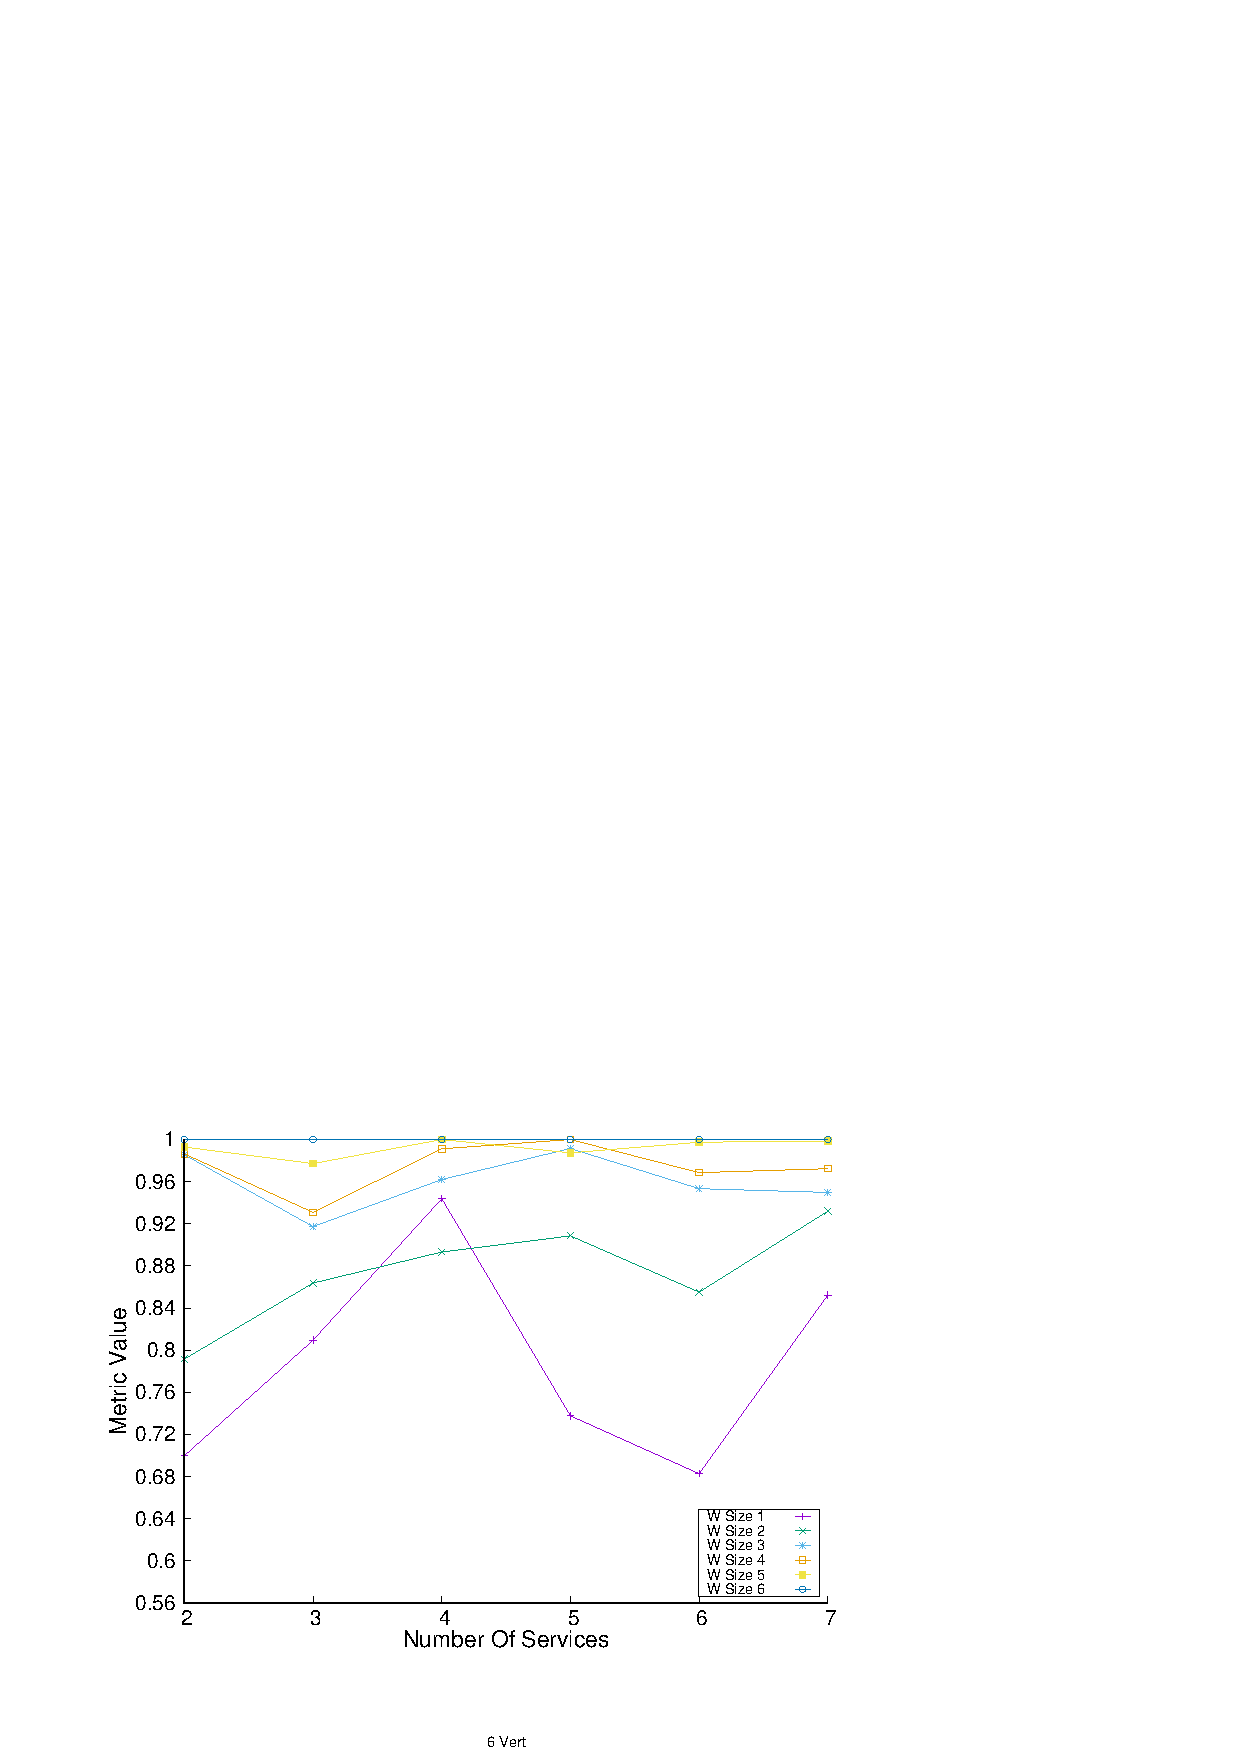
\includegraphics[width=\textwidth]{Images/graphs/window_quality_performance_diff_perce_n7_s7_20_100_n6}
    \caption{\wide 6 vertices}
    \label{fig:quality_window_perce_wide_6n}
  \end{subfigure}
  \hfill
  \begin{subfigure}{0.45\textwidth}
    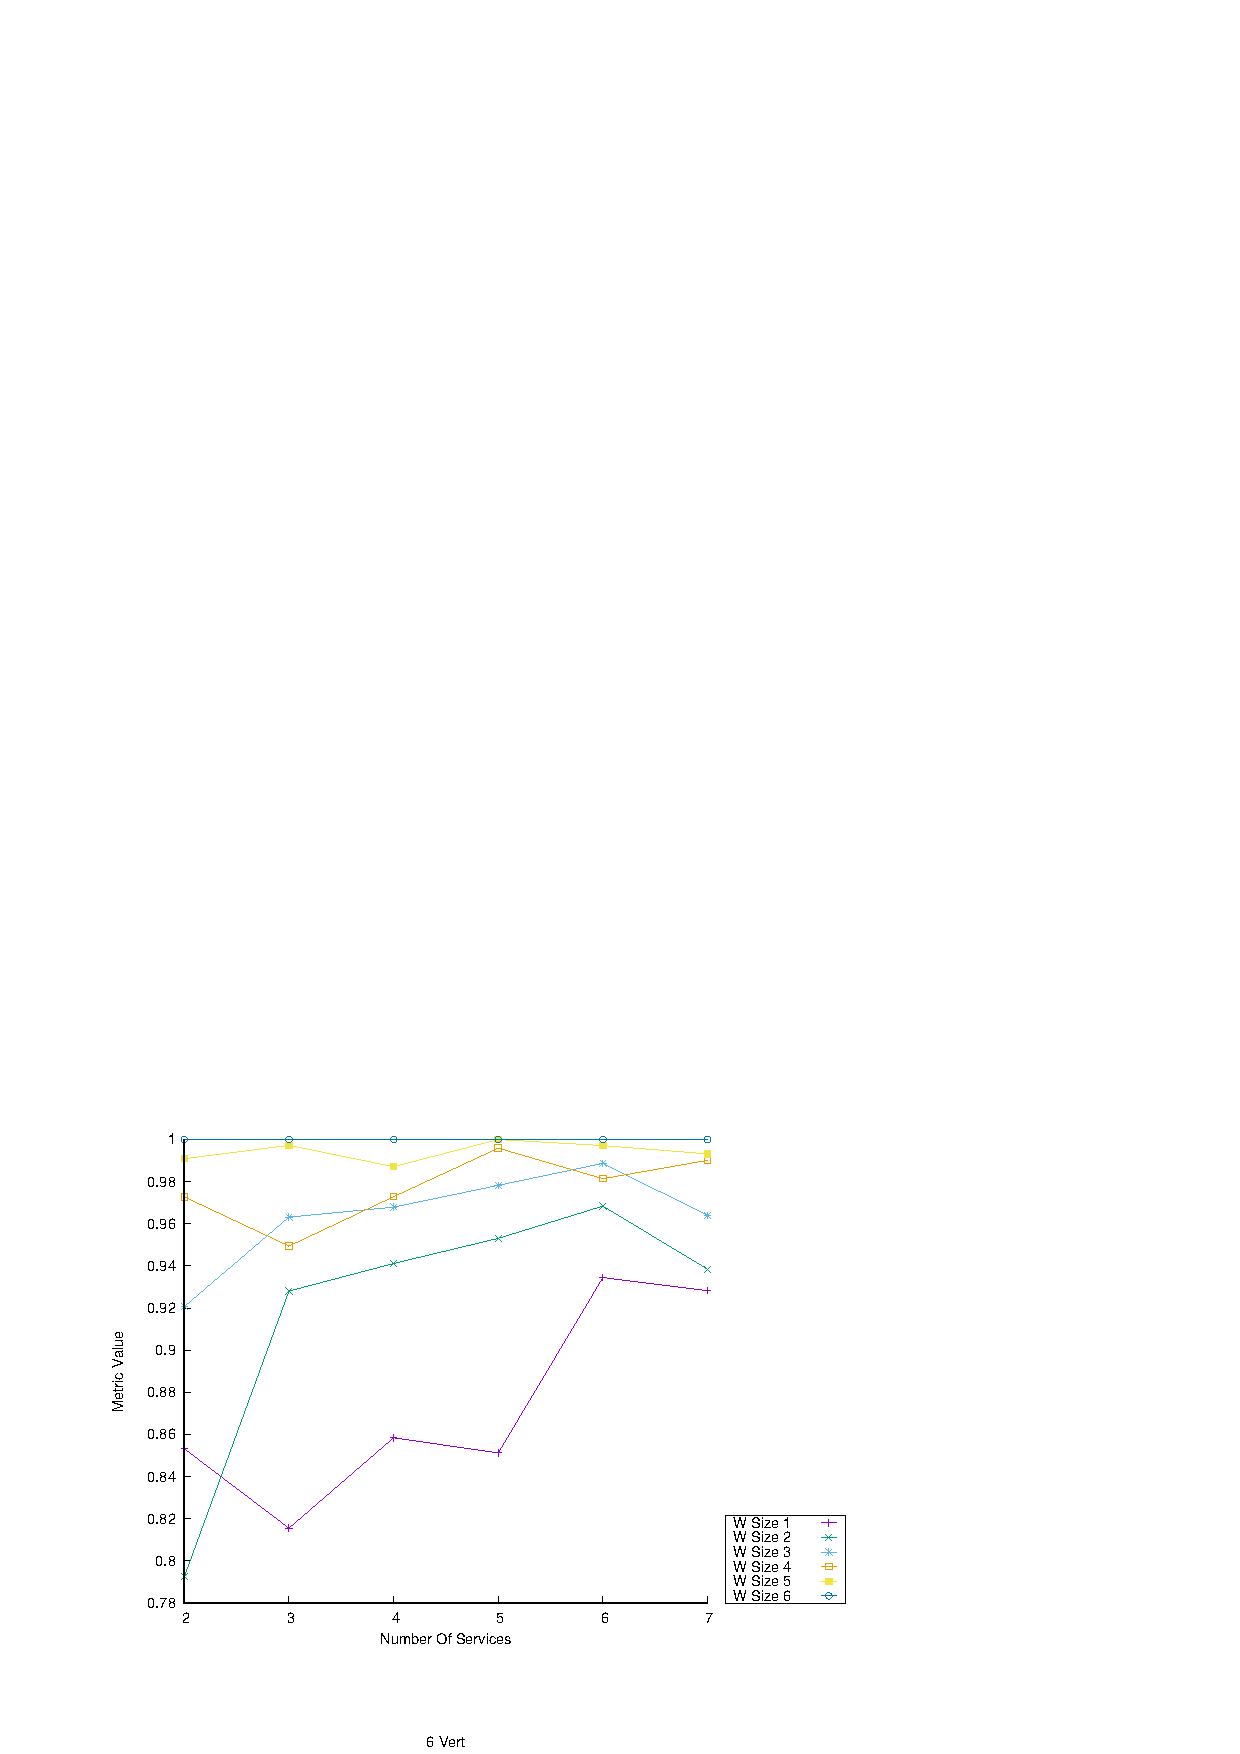
\includegraphics[width=\textwidth]{Images/graphs/window_quality_performance_diff_perce_n7_s7_50_89_n6}
    \caption{\average 6 vertices}
    \label{fig:quality_window_average_perce_6n}
  \end{subfigure}
  \begin{subfigure}{0.45\textwidth}
    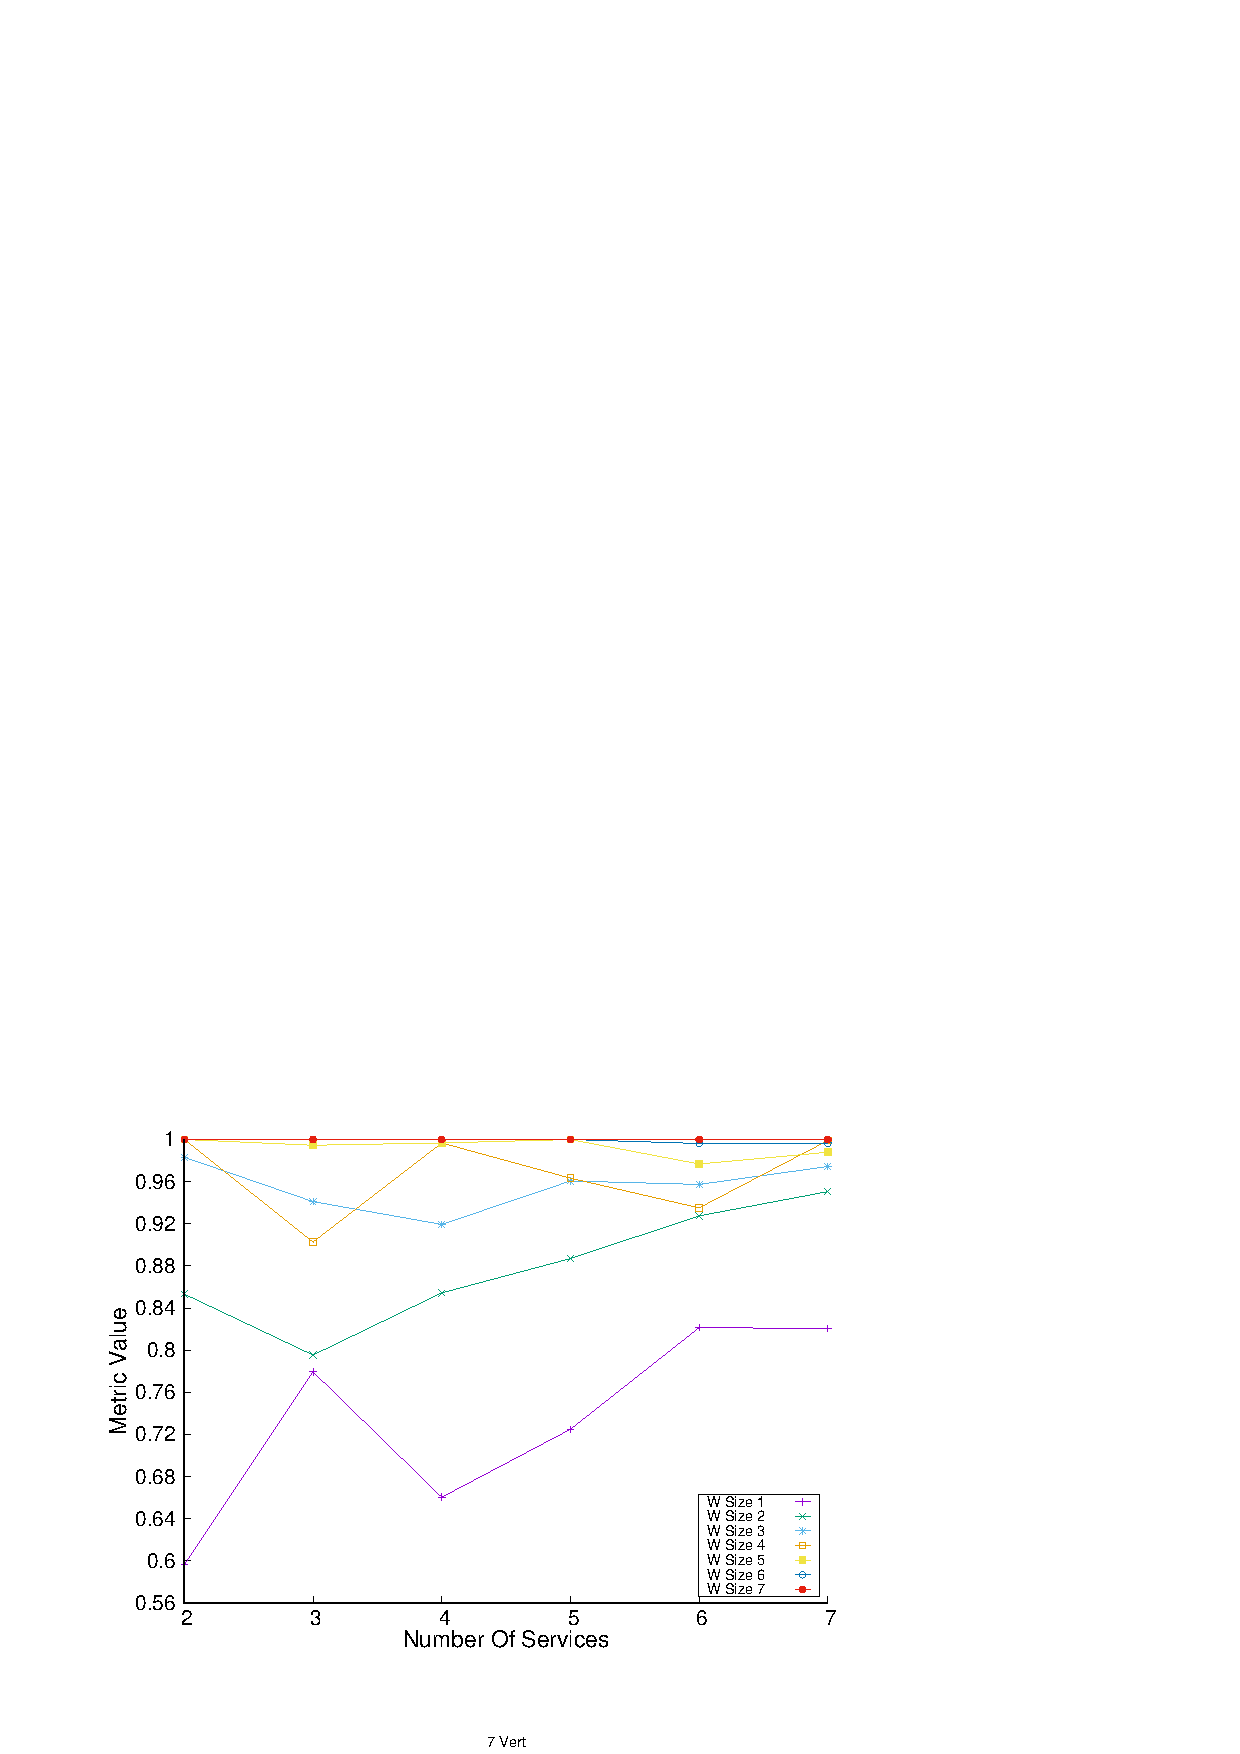
\includegraphics[width=\textwidth]{Images/graphs/window_quality_performance_diff_perce_n7_s7_20_100_n7}
    \caption{\wide 7 vertices}
    \label{fig:quality_window_perce_wide_7n}
  \end{subfigure}
  \hfill
  \begin{subfigure}{0.45\textwidth}
    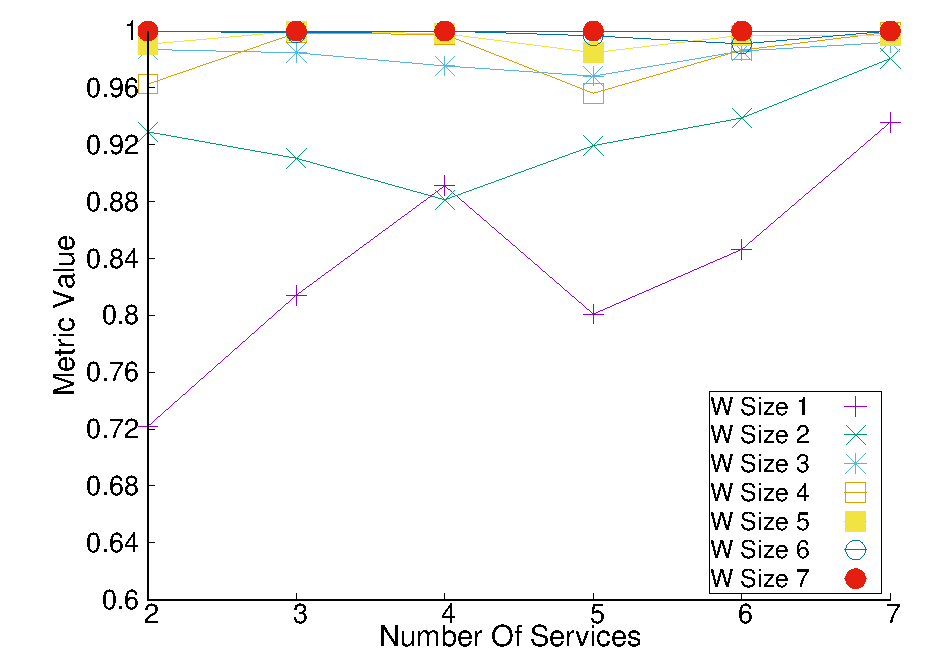
\includegraphics[width=\textwidth]{Images/graphs/window_quality_performance_diff_perce_n7_s7_50_89_n7}
    \caption{\average 7 vertices}
    \label{fig:quality_window_average_perce_7n}
  \end{subfigure}
  \caption{Evaluation of Quality Using the \emph{Quantitative} Metric in a \wide (\cref{fig:quality_window_perce_wide_3n,fig:quality_window_perce_wide_4n,fig:quality_window_perce_wide_5n,fig:quality_window_perce_wide_6n,fig:quality_window_perce_wide_7n}) and \average (\cref{fig:quality_window_average_perce_3n,fig:quality_window_average_perce_4n,fig:quality_window_average_perce_5n,fig:quality_window_average_perce_6n,fig:quality_window_average_perce_7n}) Profile Configuration.}  \label{fig:quality_window_perce}
\end{figure}


\begin{figure}[H]
  % \centering
  \begin{subfigure}{0.45\textwidth}
    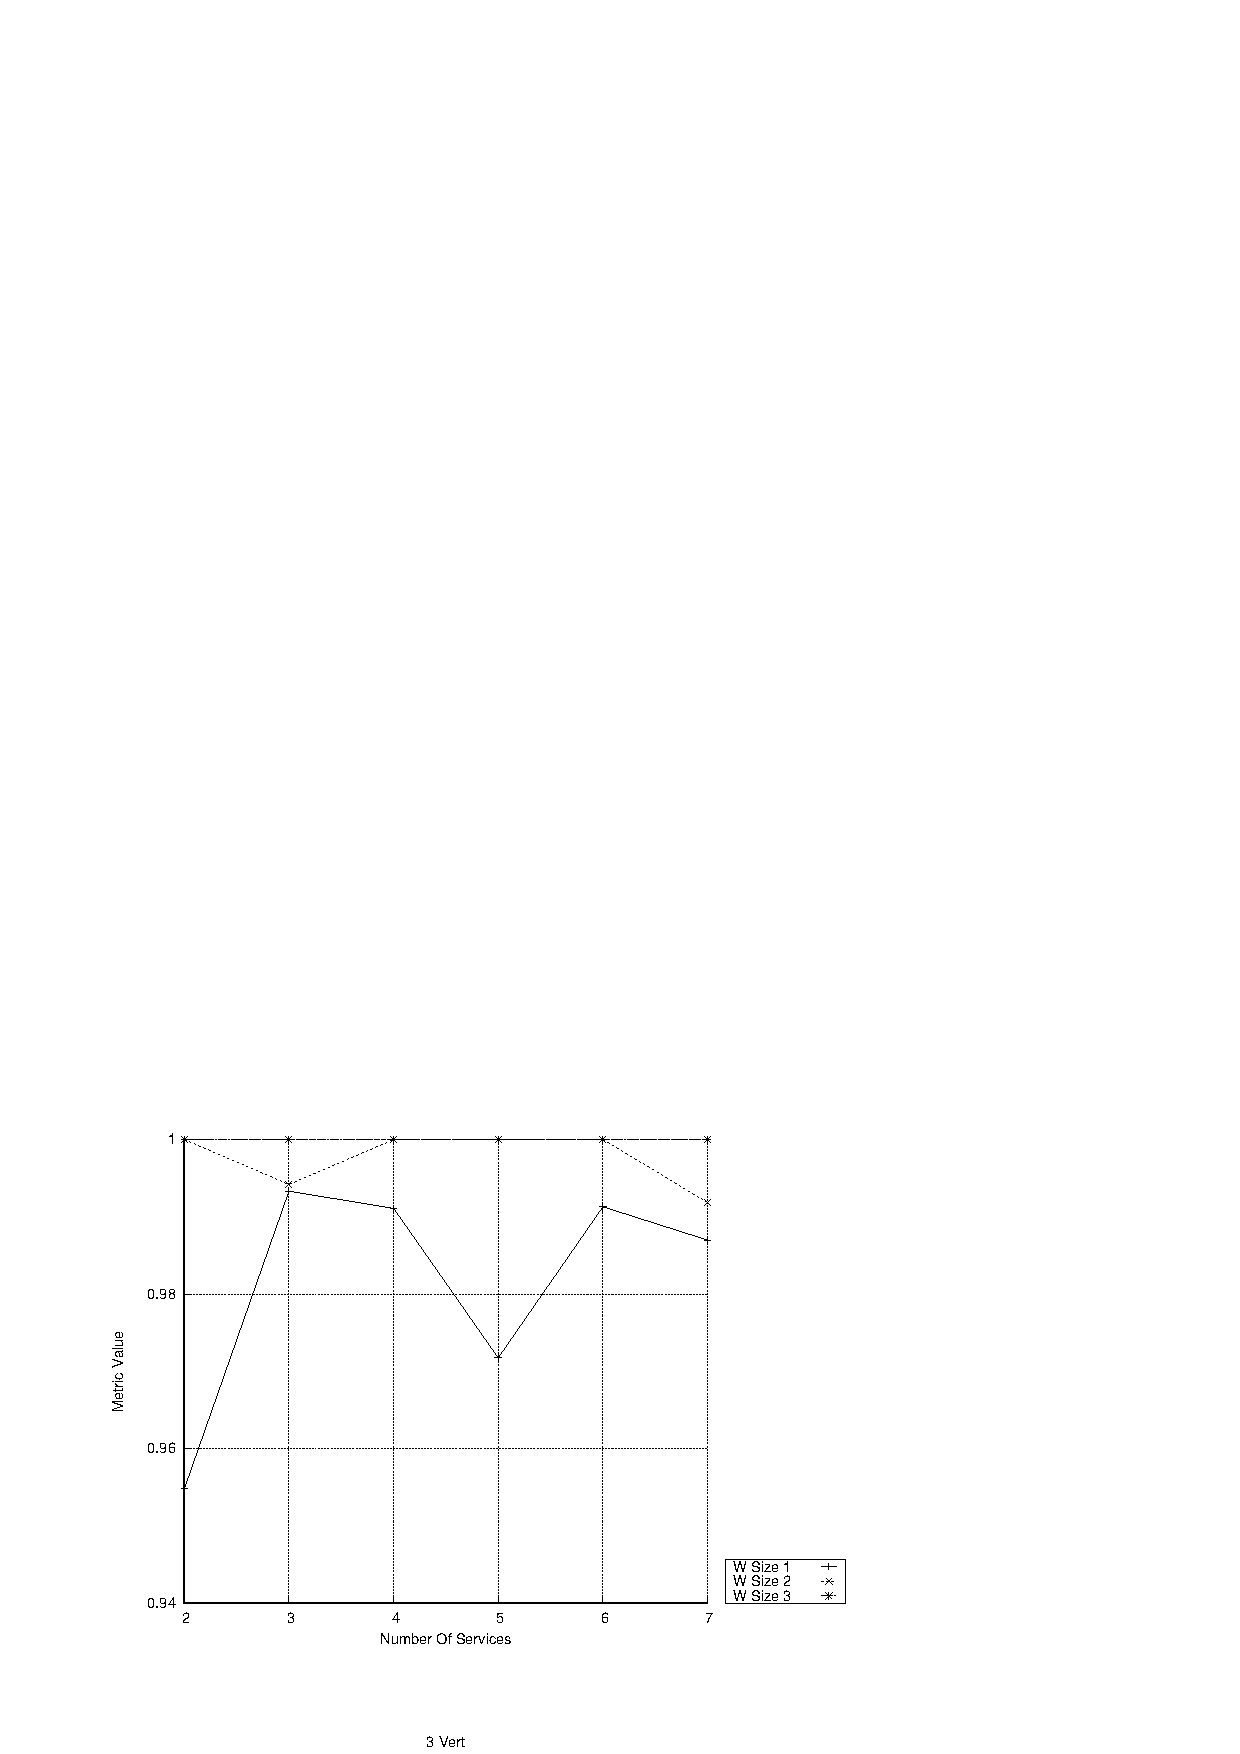
\includegraphics[width=\textwidth]{Images/graphs/window_quality_performance_diff_qual_n7_s7_20_100_n3}
    \caption{\wide 3 vertices}
    \label{fig:quality_window_wide_qualitative_n3}
  \end{subfigure}
  \hfill
  \begin{subfigure}{0.45\textwidth}
    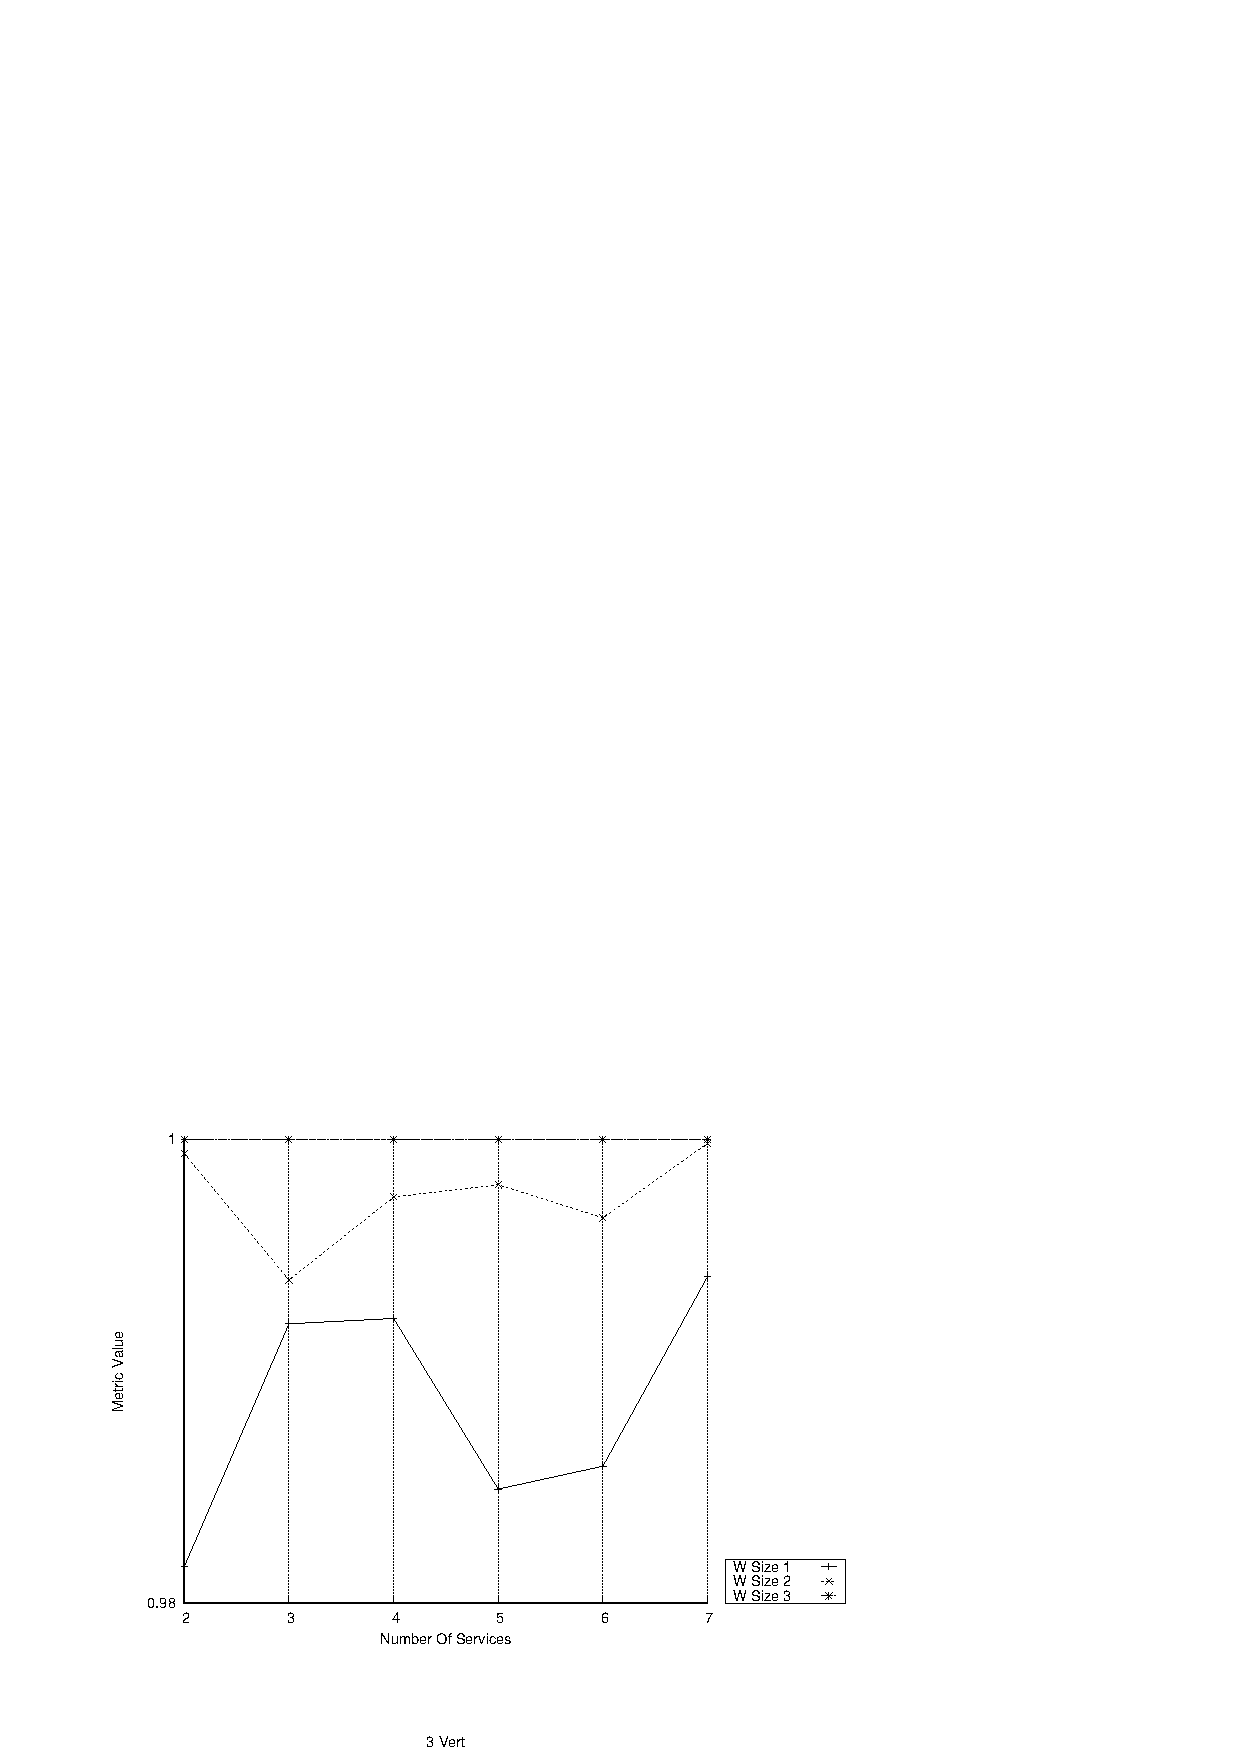
\includegraphics[width=\textwidth]{Images/graphs/window_quality_performance_diff_qual_n7_s7_50_80_n3}
    \caption{\average 3 vertices}
    \label{fig:quality_window_average_qualitative_n3}
  \end{subfigure}
  \begin{subfigure}{0.45\textwidth}
    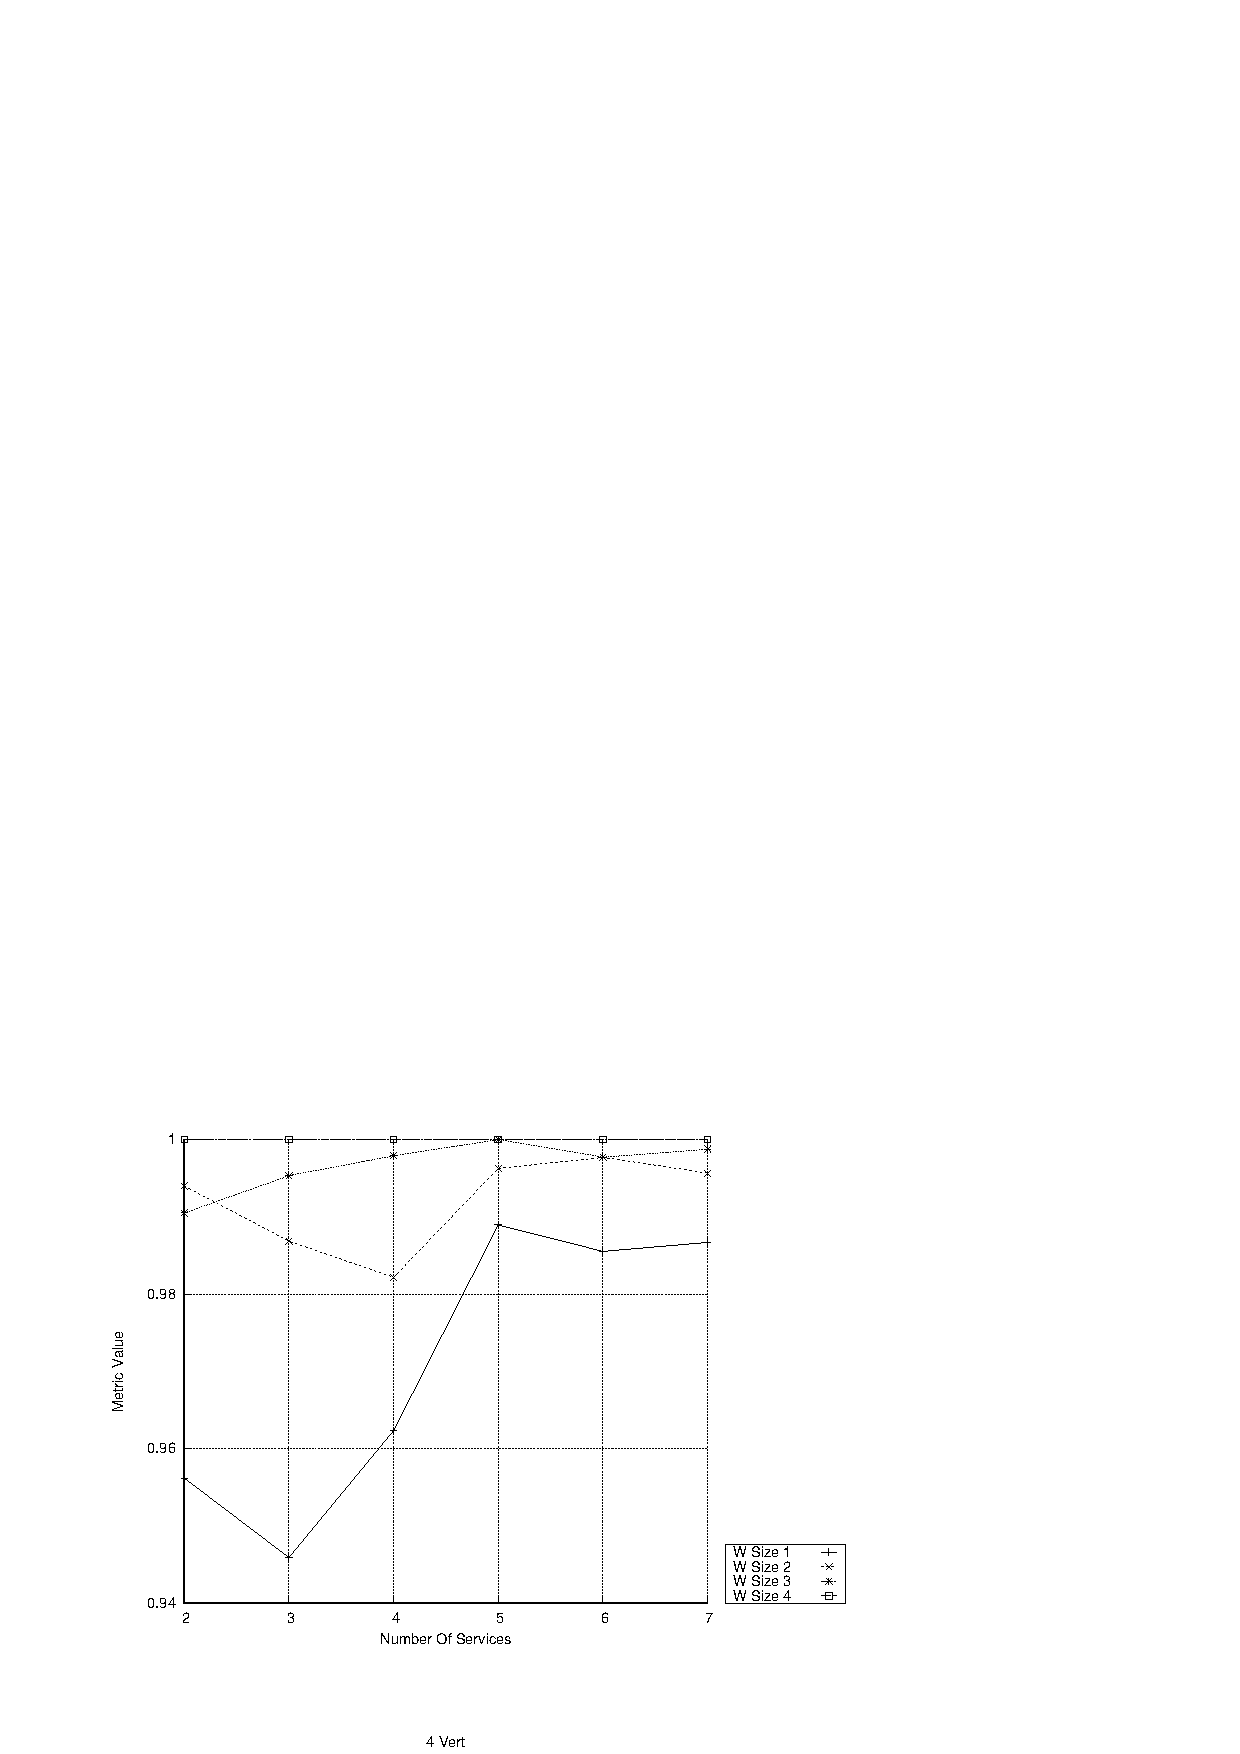
\includegraphics[width=\textwidth]{Images/graphs/window_quality_performance_diff_qual_n7_s7_20_100_n4}
    \caption{\wide 4 vertices}
    \label{fig:quality_window_wide_qualitative_n4}
  \end{subfigure}
  \hfill
  \begin{subfigure}{0.45\textwidth}
    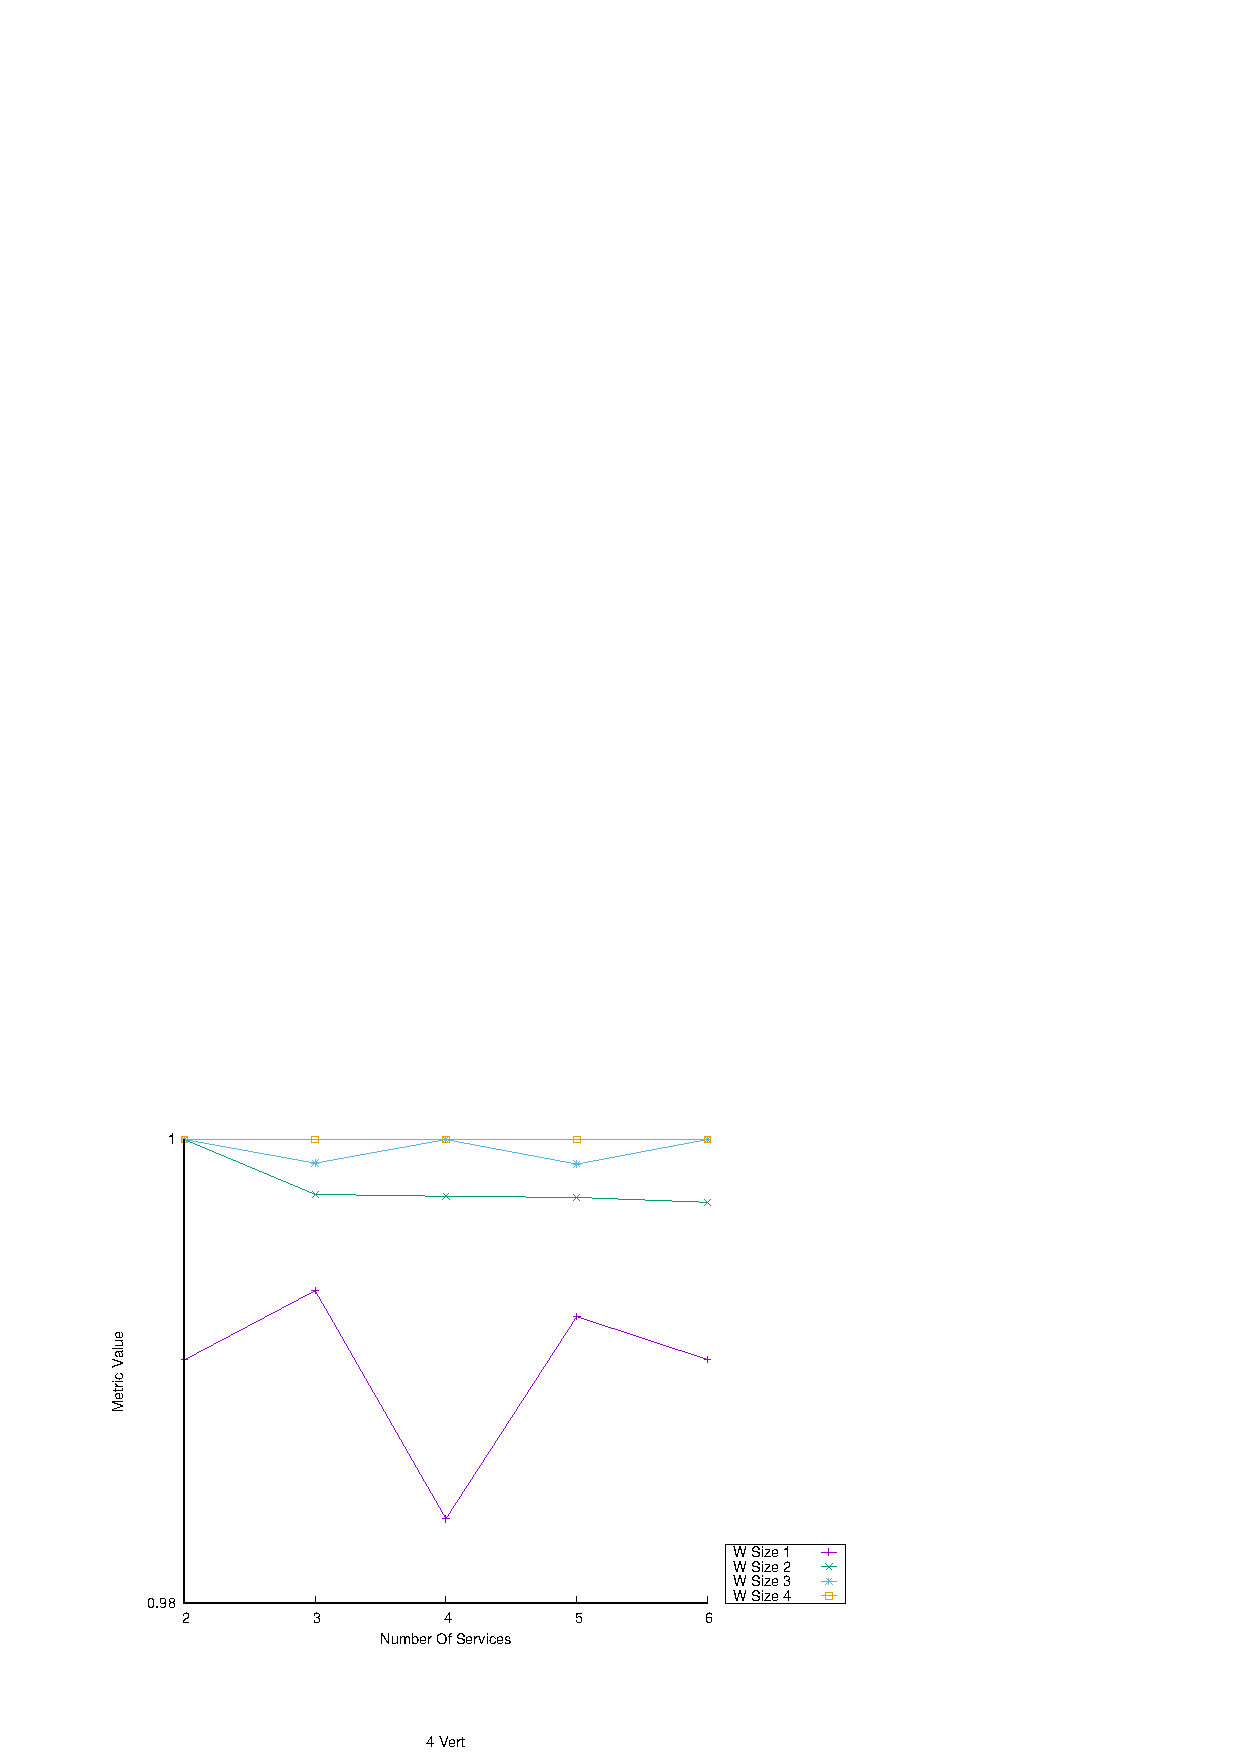
\includegraphics[width=\textwidth]{Images/graphs/window_quality_performance_diff_qual_n7_s7_50_80_n4}
    \caption{\average 4 vertices}
    \label{fig:quality_window_average_qualitative_n4}
  \end{subfigure}
  \hfill
  \begin{subfigure}{0.45\textwidth}
    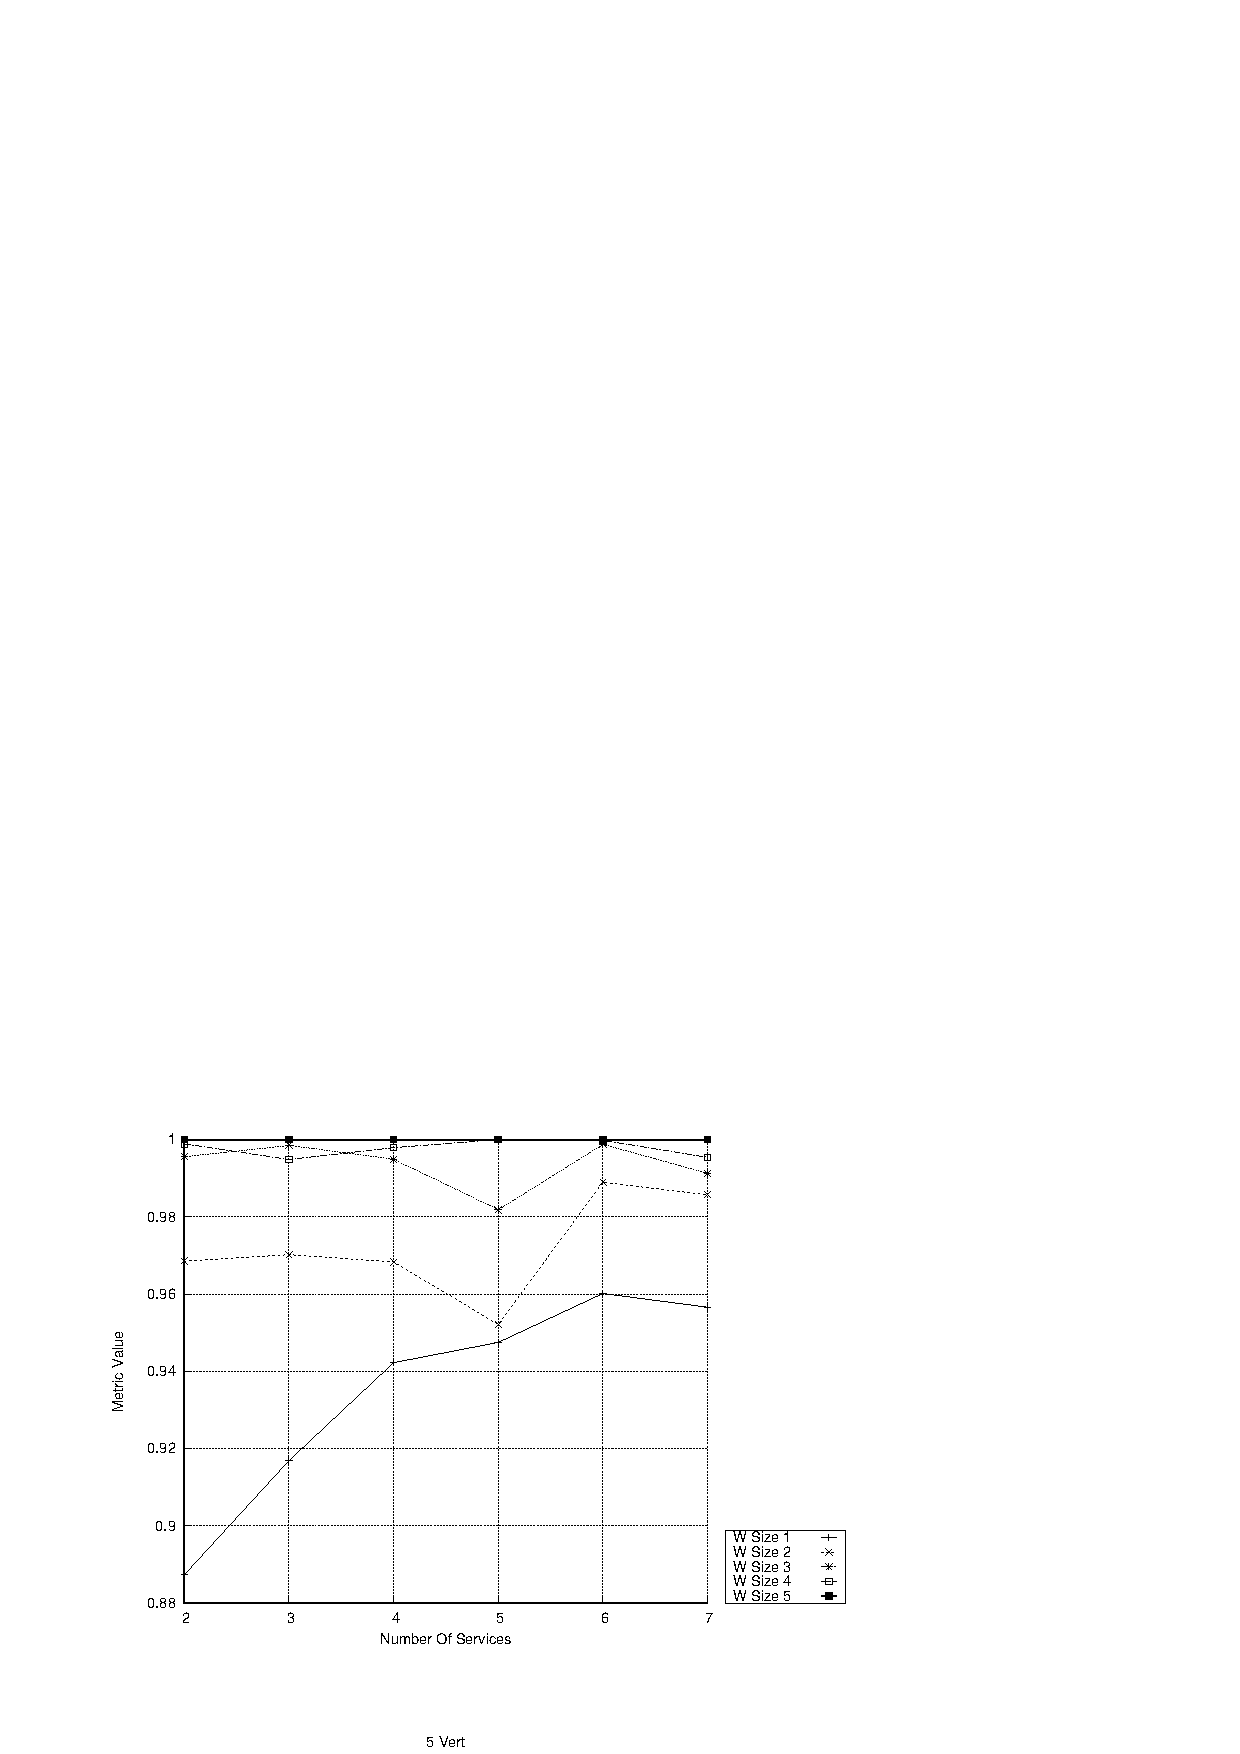
\includegraphics[width=\textwidth]{Images/graphs/window_quality_performance_diff_qual_n7_s7_20_100_n5}
    \caption{\wide 5 vertices}
    \label{fig:quality_window_wide_qualitative_n5}
  \end{subfigure}
  \hfill
  \begin{subfigure}{0.45\textwidth}
    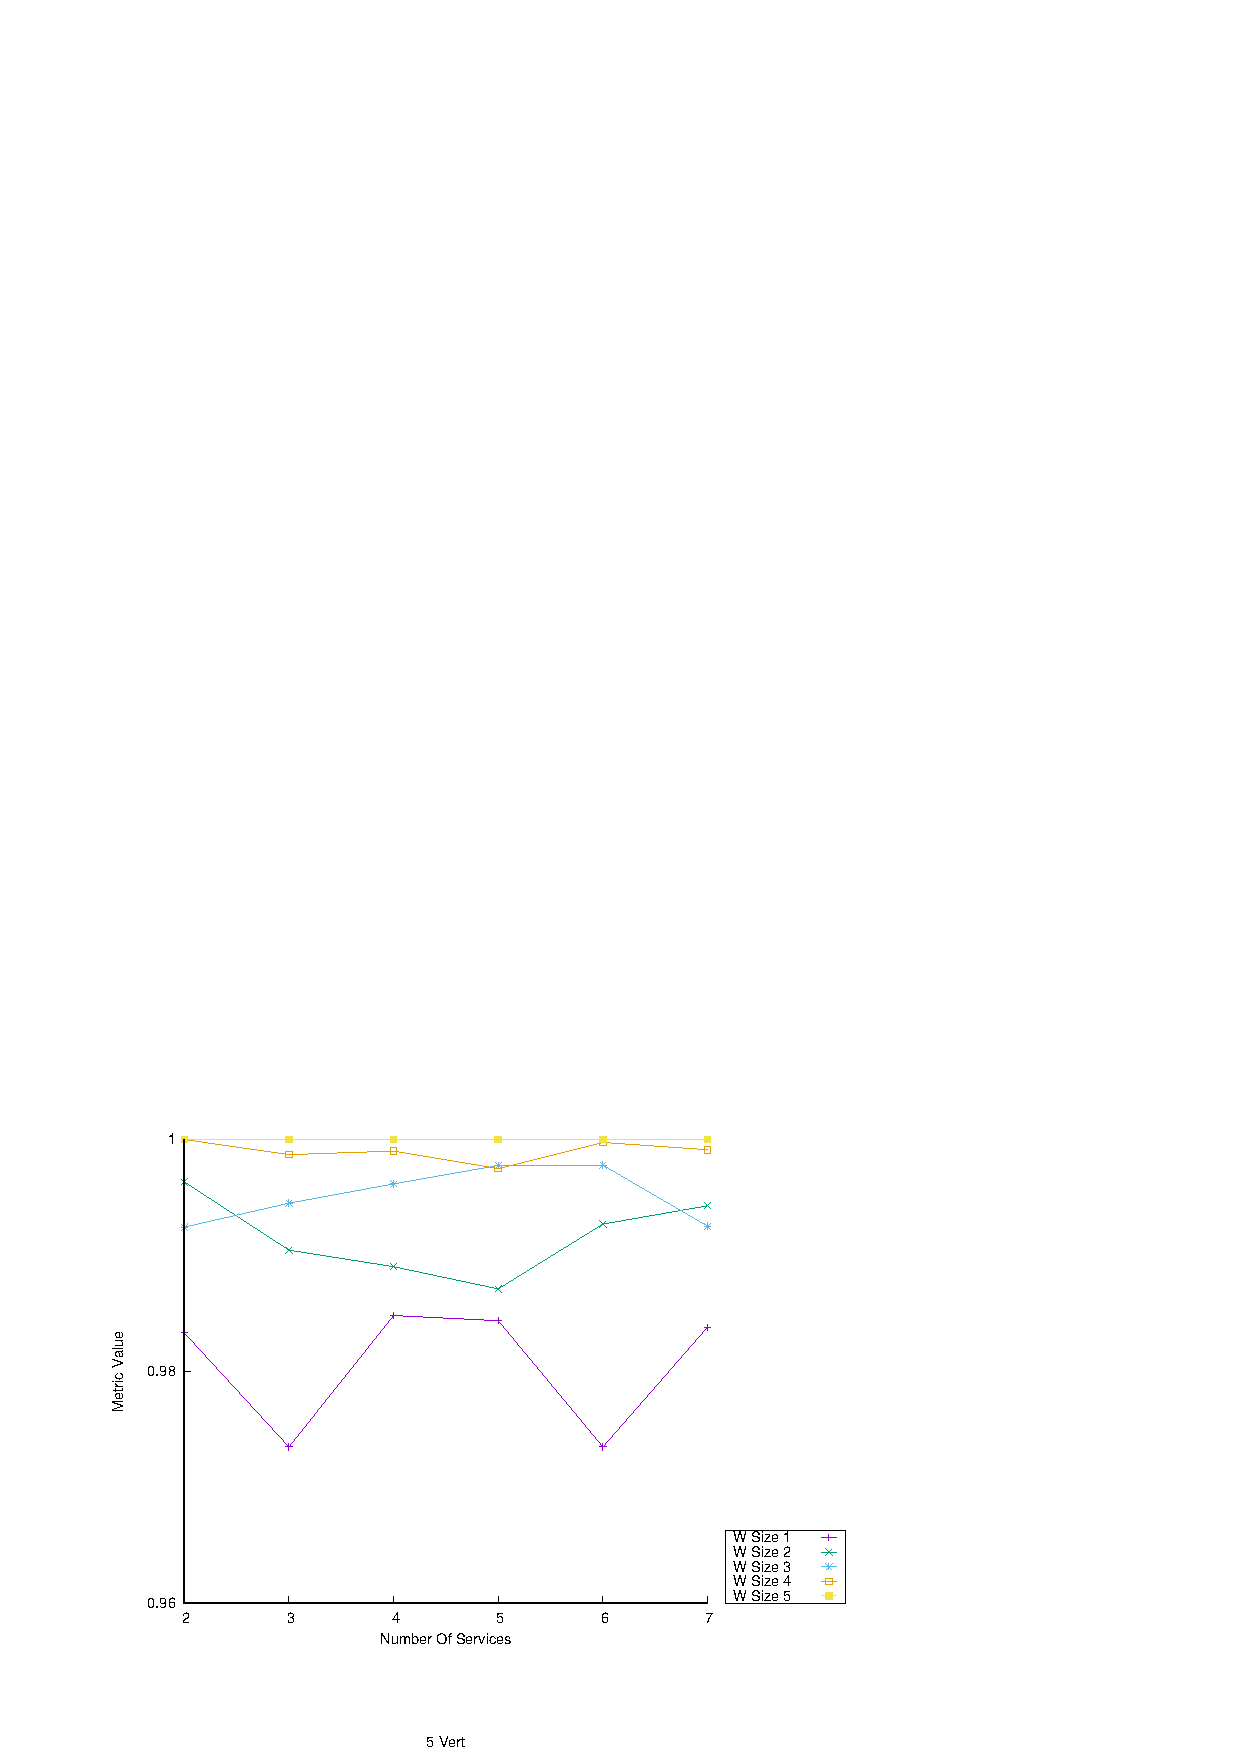
\includegraphics[width=\textwidth]{Images/graphs/window_quality_performance_diff_qual_n7_s7_50_80_n5}
    \caption{\average 5 vertices}
    \label{fig:quality_window_average_qualitative_n5}
  \end{subfigure}
  \begin{subfigure}{0.45\textwidth}
    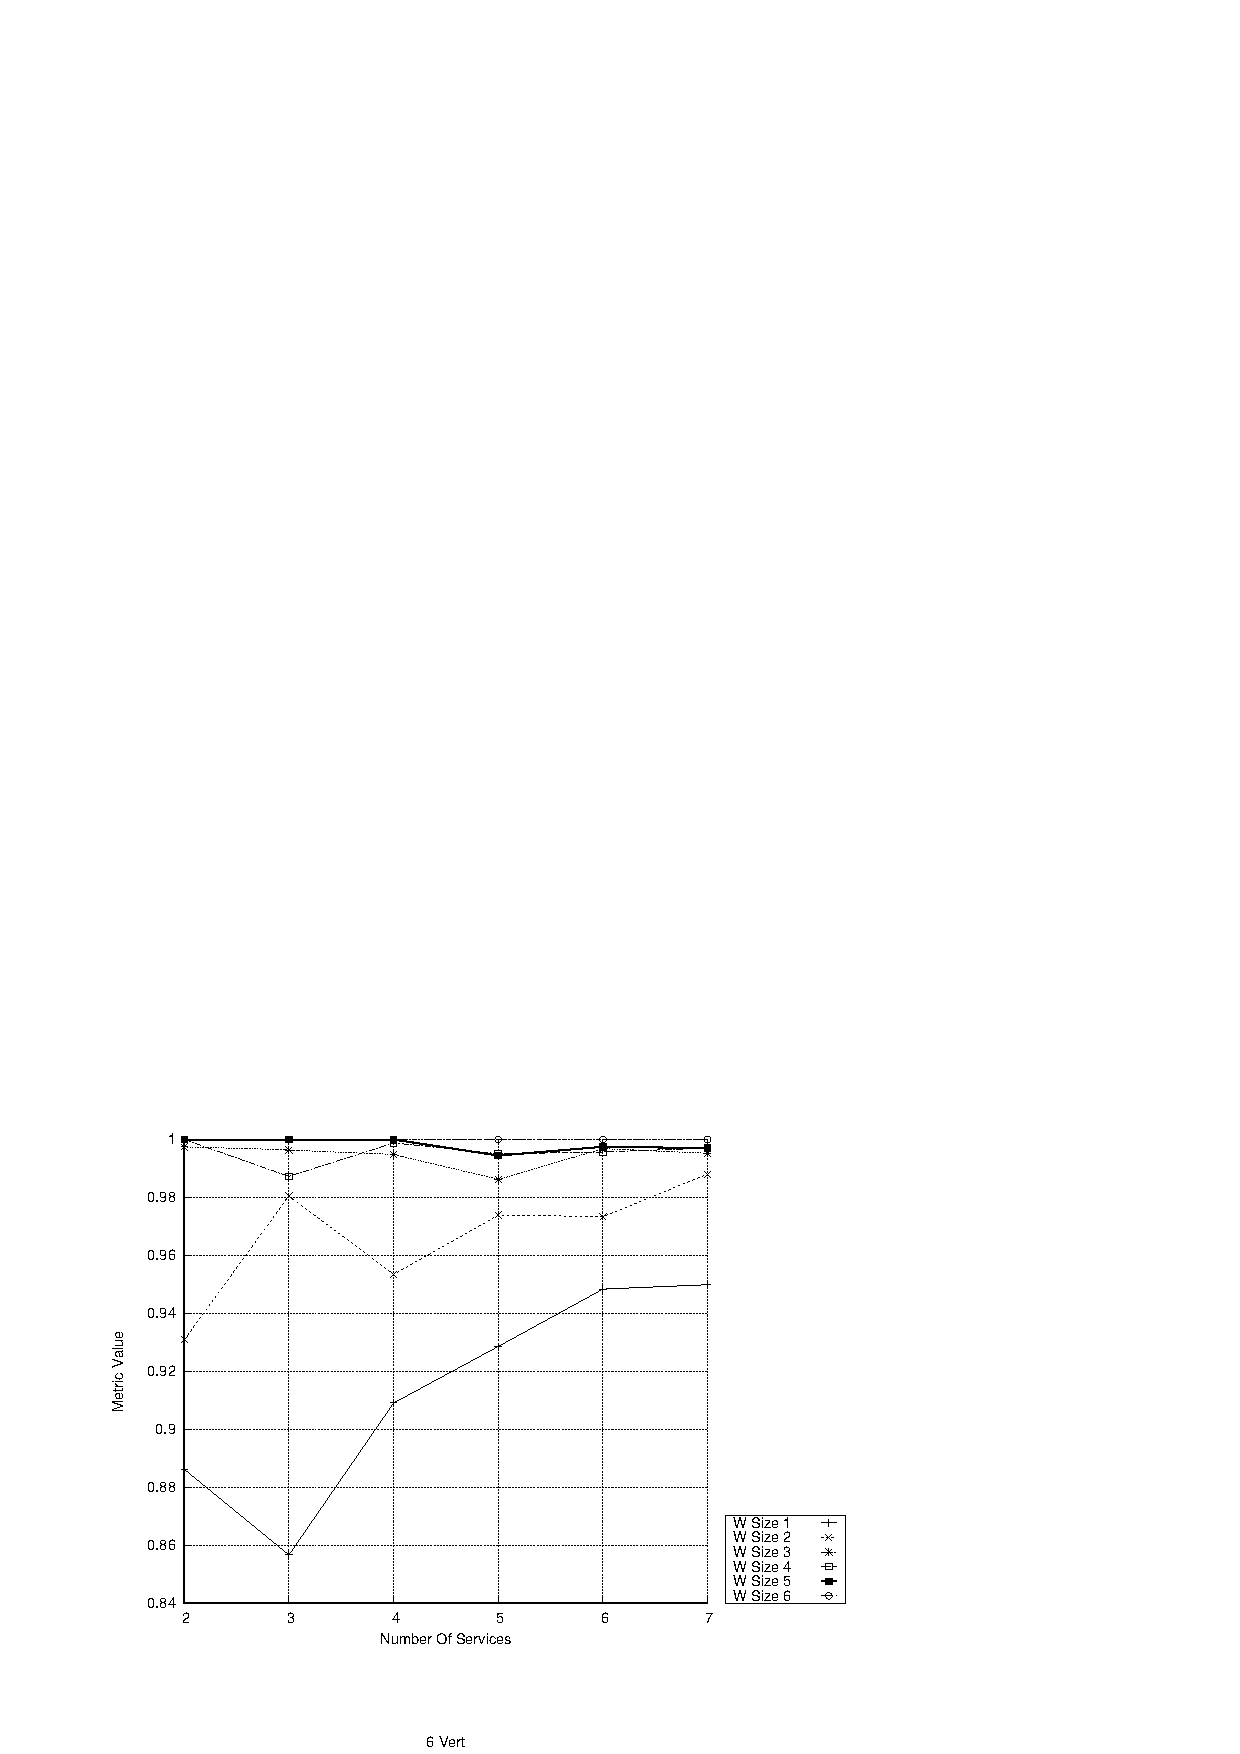
\includegraphics[width=\textwidth]{Images/graphs/window_quality_performance_diff_qual_n7_s7_20_100_n6}
    \caption{\wide 6 vertices}
    \label{fig:quality_window_wide_qualitative_n6}
  \end{subfigure}
  \hfill
  \begin{subfigure}{0.45\textwidth}
    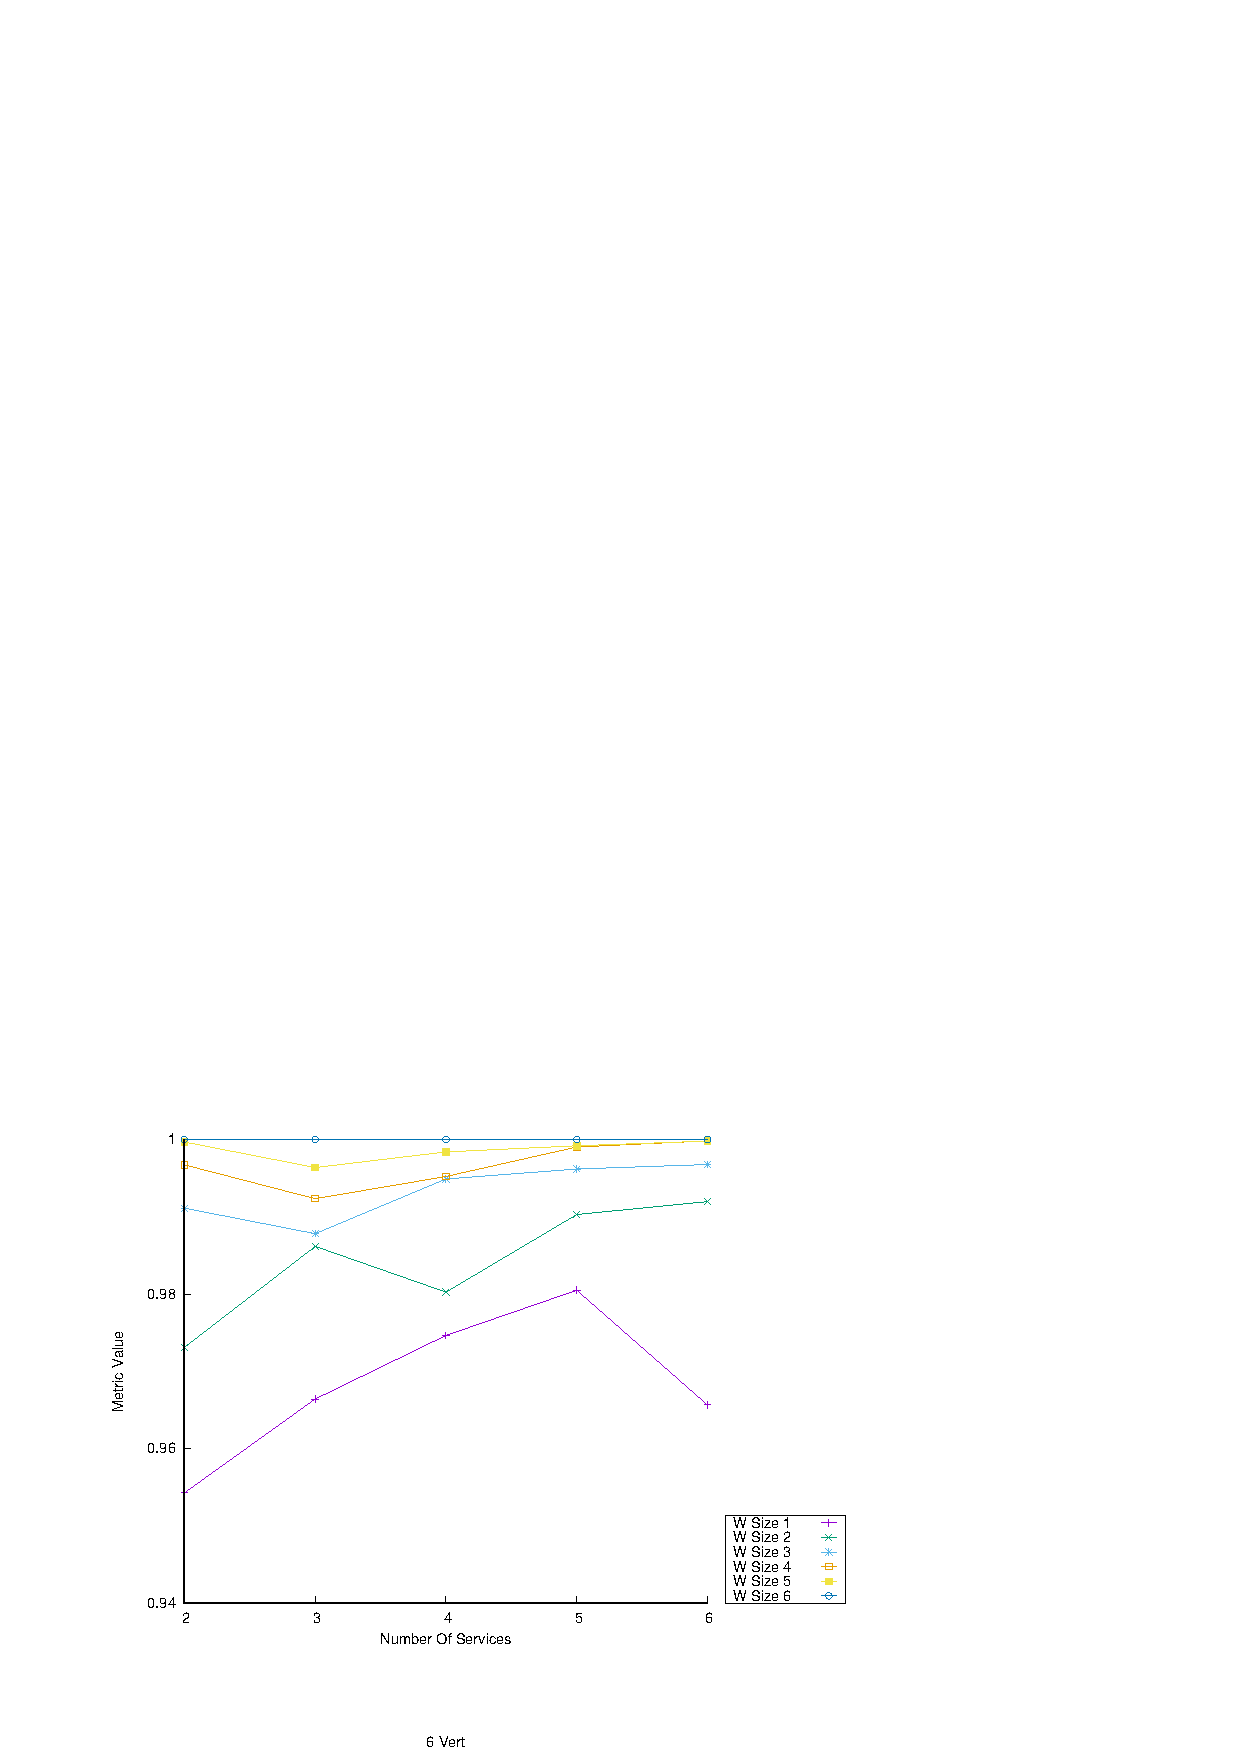
\includegraphics[width=\textwidth]{Images/graphs/window_quality_performance_diff_qual_n7_s7_50_80_n6}
    \caption{\average 6 vertices}
    \label{fig:quality_window_average_qualitative_n6}
  \end{subfigure}
  \hfill
  \begin{subfigure}{0.45\textwidth}
    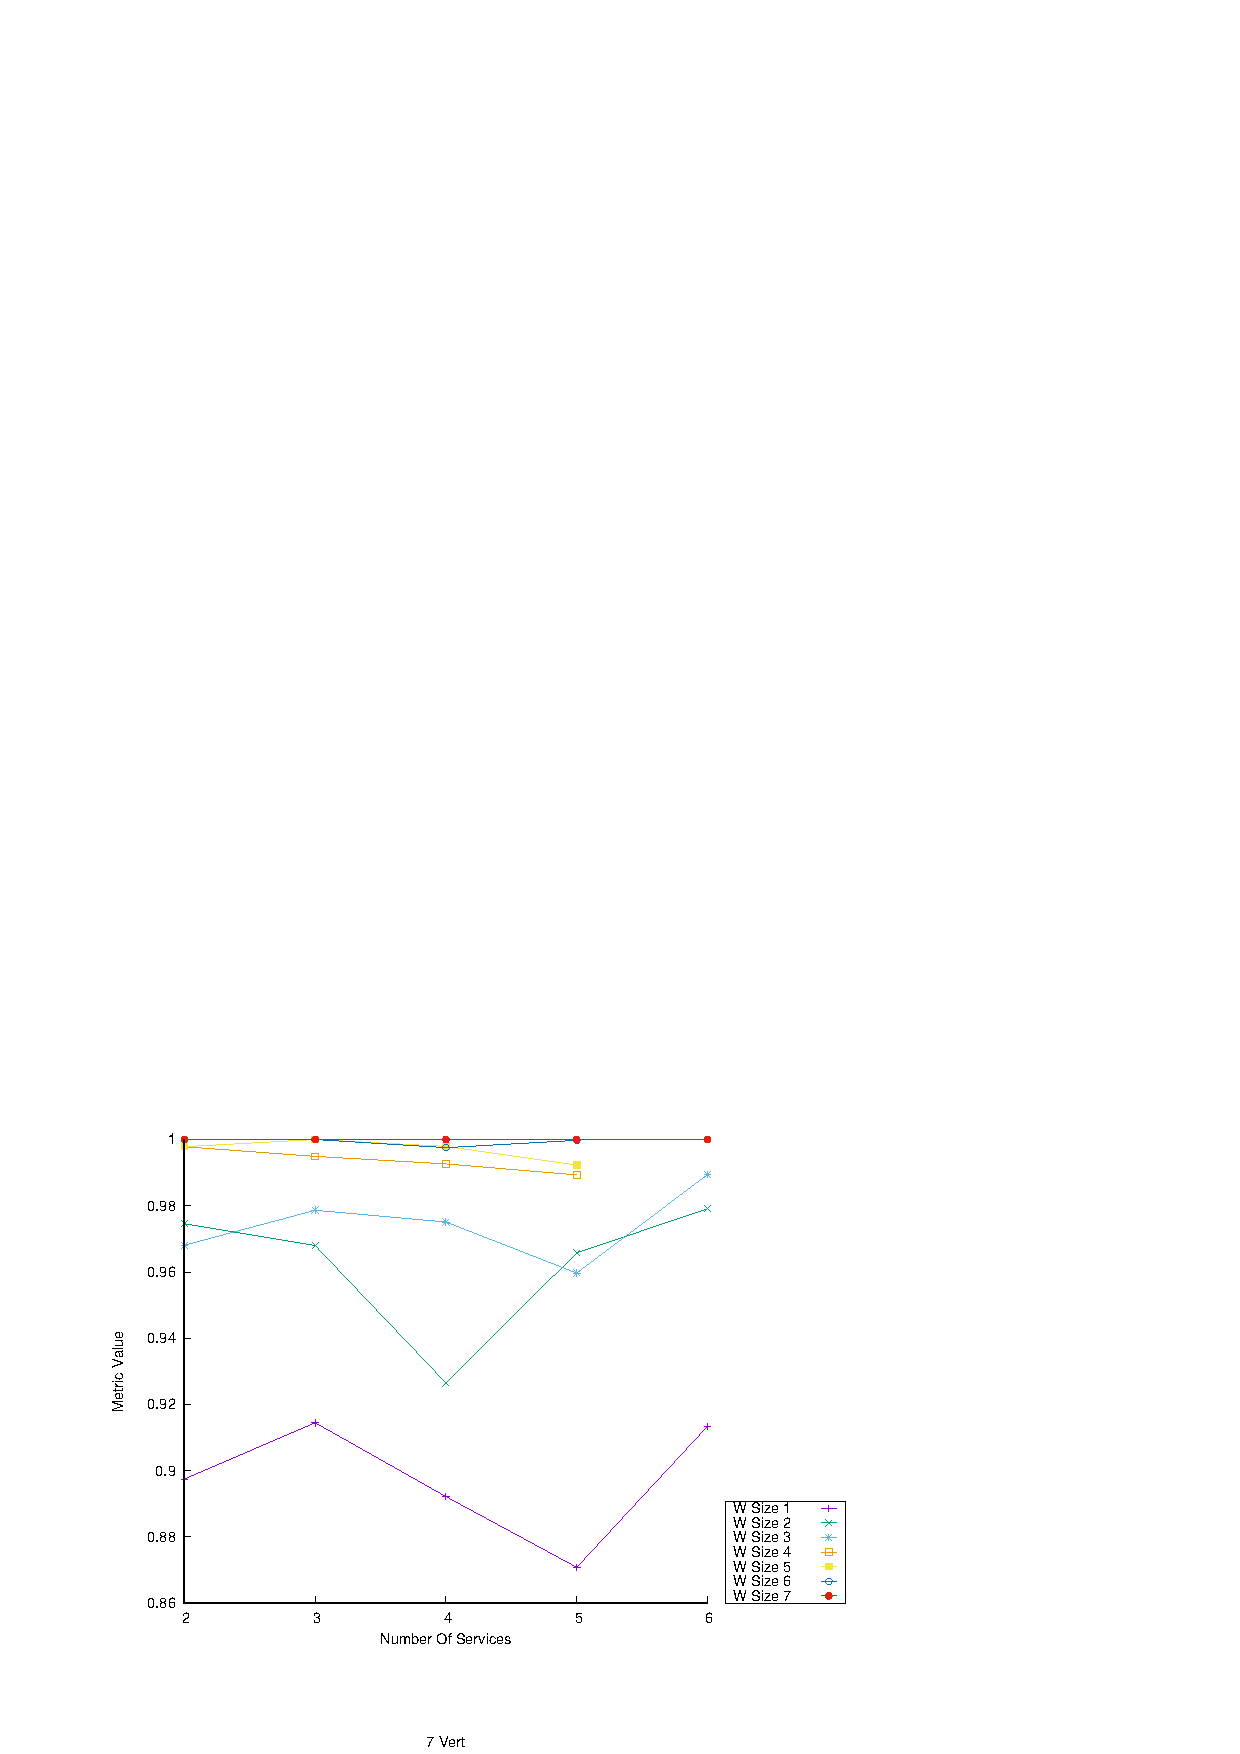
\includegraphics[width=\textwidth]{Images/graphs/window_quality_performance_diff_qual_n7_s7_20_100_n7}
    \caption{\wide 7 vertices}
    \label{fig:quality_window_wide_qualitative_n7}
  \end{subfigure}
  \hfill
  \begin{subfigure}{0.45\textwidth}
    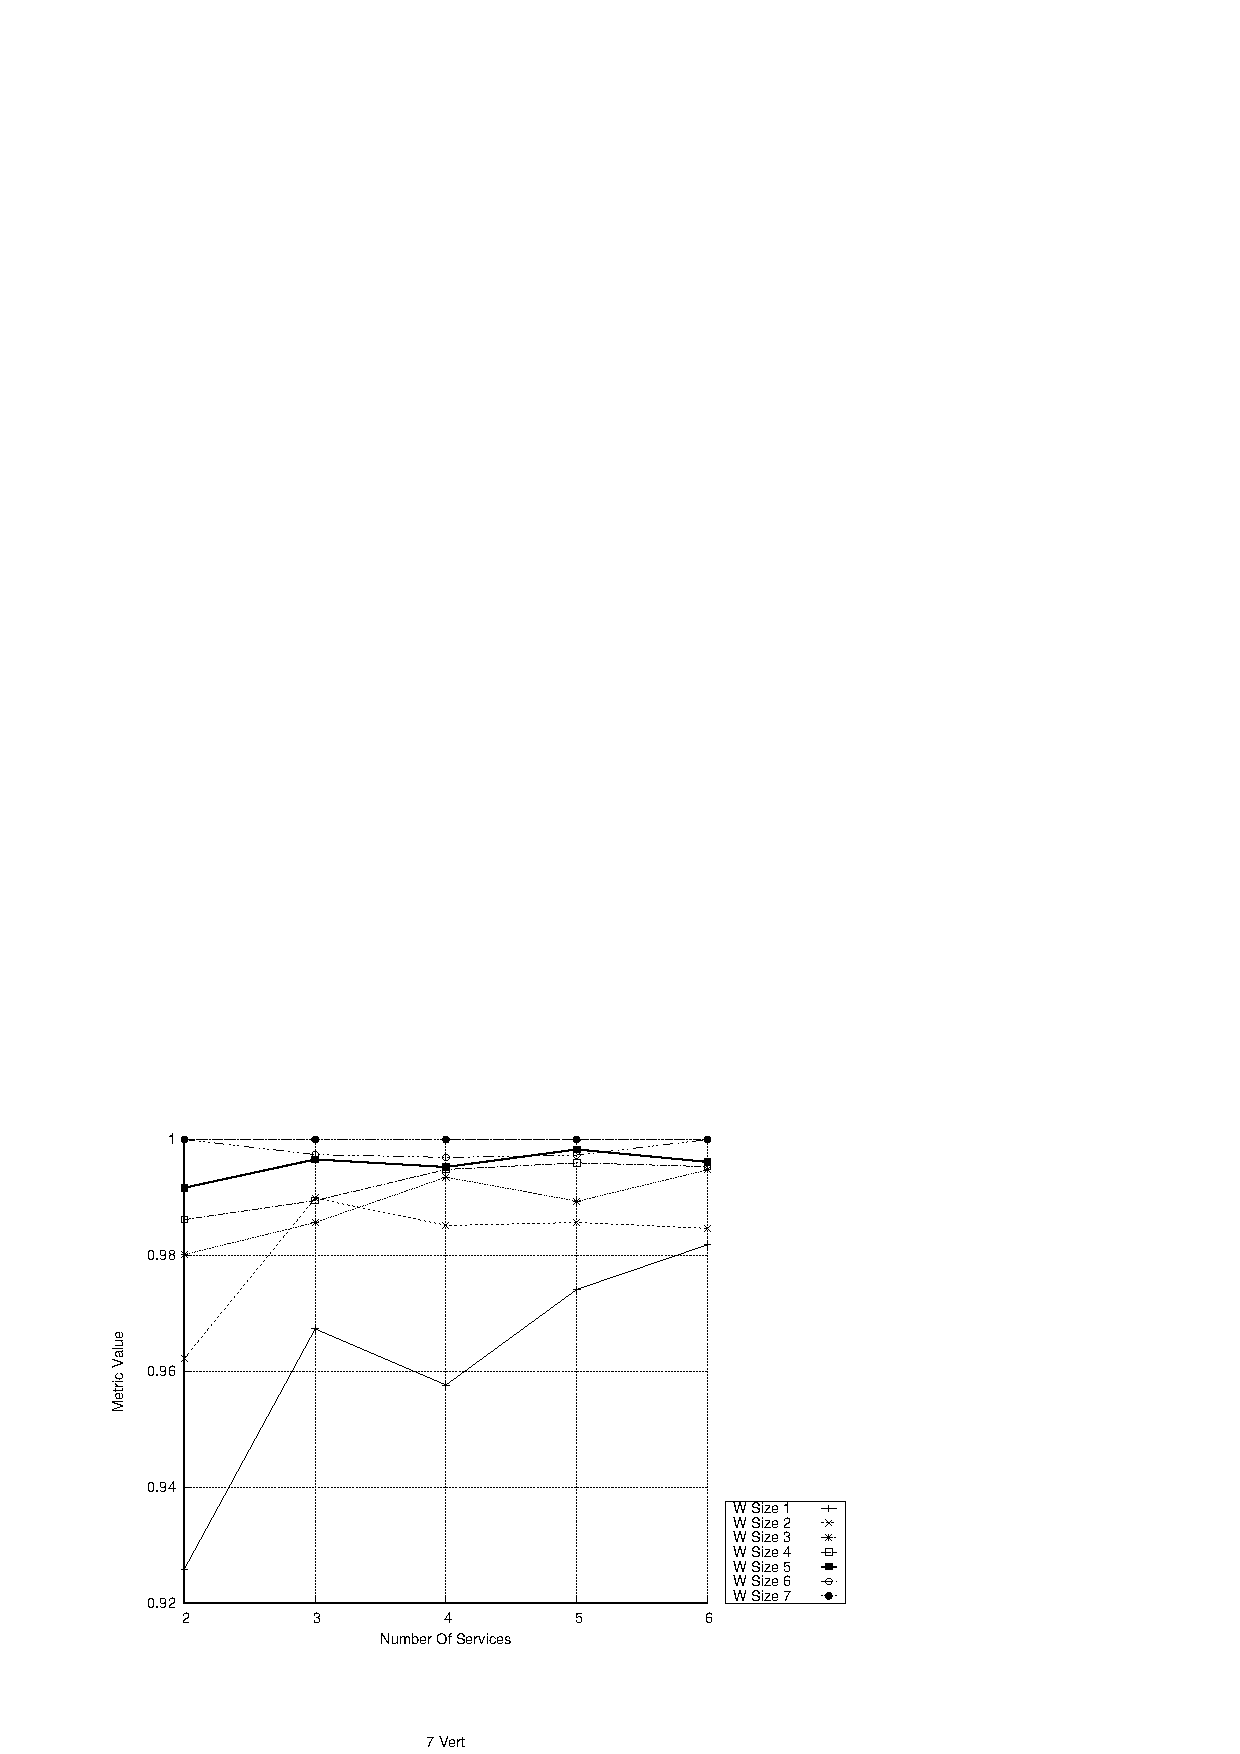
\includegraphics[width=\textwidth]{Images/graphs/window_quality_performance_diff_qual_n7_s7_50_80_n7}
    \caption{\average 7 vertices}
    \label{fig:quality_window_average_qualitative_n7}
  \end{subfigure}

  \caption{Evaluation of Quality Using the \emph{Qualitative} Metric in a \wide (\cref{fig:quality_window_wide_qualitative_n3,fig:quality_window_wide_qualitative_n4,fig:quality_window_wide_qualitative_n5,fig:quality_window_wide_qualitative_n6,fig:quality_window_wide_qualitative_n7}) and \average (\cref{fig:quality_window_average_qualitative_n3,fig:quality_window_average_qualitative_n4,fig:quality_window_average_qualitative_n5,fig:quality_window_average_qualitative_n6,fig:quality_window_average_qualitative_n7}) Profile Configuration.}  \label{fig:quality_window_qualitative}

\end{figure}


